\chapter{Applying Saddle Point Construction in Complex Systems} %% change
\label{chapter_4} %% change
\graphicspath{ {./chapter-4/figures/} }  %% change
\captionsetup[figure]{labelfont=bf}
\captionsetup{margin=1.5em}
\captionsetup[table]{labelfont=bf}

% The following annotation is customary for chapter which have already been
% published as a paper.
% \blfootnote{Parts of this chapter have been published in Annalen der Physik \textbf{324}, 289 (1906) \cite{LinWang2011}.}

%% It is only necessary to list the authors if multiple people contributed
%% significantly to the chapter.
%\authors{Albert {\titleshape Einstein}}

%% The '0pt' option ensures that no extra vertical space follows this epigraph,
%% since there is another epigraph after it.
% \epigraph[0pt]{
%   The proof of the pudding is in the eating.}

% \epigraph{
%     Sample quotes
% }{author}

% \begin{abstract}
% Previous researches have shown that different solutions of the optical system can be found using saddle point based method for some simplified cases\cite{PascalTriplet2009}. It is important, however, to study whether the saddle point based method still perform well in practical lens design problems. To study this, we chose to start with a relative simple example.
% \end{abstract}

% %% Start the actual chapter on a new page.
% \newpage

How to apply SPC in a real design problem?  
Previous investigations have shown that in an idealized lens design problem, where the structure of the landscape is determined by spherical aberration, all the solutions in the design landscape can be obtained via SPC \cite{PascalTriplet2009}. A detailed study of the design network of a simple wide angle pin-hole lens \cite{HouSimple16} shows that SPC is effective to escape from poor local minima and to reach to the global minimum. In a specific case, SPC is able to find all the solutions found in the design landscape with other methods. A thorough study of the design landscape of a complicated system will be quite difficult, but the above results for simple systems give us confidence in the ability of SPC to find new good solutions for complicated lens systems as well. 

%%%%%%%%%%%%%%%%%%%%%%%%%%%%%%%%%%%%%%%%%%% Section 1 %%%%%%%%%%%%%%%%%%%%%%%%%%%%%%%%%%%%%%%
\section{Introduction}

Systems with limited amount of curvature variables are easier to be studied using saddle point construction. Given problem with small amount of variables, it is possible to investigate the solutions in the design landscape using different methods. Therefore, the quality of the solutions from saddle point construction can be evaluated. In practical optical design, especially difficult design tasks, complex systems are usually designed, where large number of lenses is used. For example, a patented objective, which will be shown later, consists of more than twenty lenses in order to achieve nanometer accuracy. These objectives are used in the semiconductor industry to produce integrated chips \cite{Matsuyama2006_LithoHis}. For these complicated optical systems, the number of possible solutions increased compared to the case of simpler systems. The complicated optical systems are also more sensitive to ray failures, which varying variables in the system can easily cause failures in ray tracing. Designing such a complex lens are usually starting from an existing design, which has similar specifications compared to the design goal. The lens is altered by the designer based on certain design guidelines \cite{LivshitsQA2013}\cite{Shafer1995_moreless}\cite{Cao2017_GroupDesign} or his/her own experience. Trial and error always evolves before obtaining a good solution. 

In this chapter, we apply the saddle point construction method in complicated design cases. For these complicated systems, it is difficult and not very practical to sort out all the minima connections in a design landscape. Nether is there enough confidence that we can find most of the solutions for a complicated systems with existing methods. Nevertheless, we can still apply the saddle point construction method to these systems to evaluate the performance of saddle point construction. The special case of saddle point construction has been used to assist the designing of complicated lenses \cite{Cao2017_GroupDesign}\cite{MarinescuSP2008}\cite{MarinescuSPS2008_p2} and the results demonstrate its possibility for finding new local minima for complicated system. The general version of the saddle point construction \cite{vanTurnhoutThesis2009} has never been described in the literature. Even though the method is not new, its application in complicated systems has not yet be studied. We have chosen three optical systems, from moderate complexity to extreme complexity, to give example on how the general version of saddle point construction can be applied in practical design situation. We will explain the difficulties encountered when handle complicated optical design, evaluating the performance of the saddle point construction method and give recommondations on how the method should be executed to achieve the best results.


\section{Investigation of a wide angle lens with six elements}
Wide angle lenses are broadly used for various applications, including photographic cameras, surveillance cameras and projectors. To increase the field of view of the system and maintain a good image quality, a certain complexity of the system is necessary. A wide angle lens with a moderate complexity is chosen here to study the performance of SPC as a switching tool. The system consists of six lenses including one cemented surface. The specifications of the lens are shown in Table \ref{table: sysspecWAL}. The maximum field of view is 120°. The overall length of the system is 38.75mm, which is small enough for integration into surveillance systems. The MTF curve shows that the modulation stays above 0.4 for 100 cycles/mm at full field of view. The system is not optimized for distortion, which can be corrected with image processing tools afterwards \cite{Sahin:18DisCorrec}.

\setlength{\arrayrulewidth}{.5mm}
\setlength{\tabcolsep}{18pt}
\renewcommand{\arraystretch}{1.2}
\begin{table}[h!]
    \centering
    \captionsetup{justification=centering}
    \caption{System specification of the wide-angle lens}
    \label{table: sysspecWAL}
    \vspace{-1em}
    \begin{tabular}{ p{20em} c }
    \hline 
    Full field of view (FOV, °) & 120\\
    Effective focal length (EFL, mm) & 3.0\\
    F Number & 2.0\\
    Overall Length (mm) & 38.75\\
    Wavelength (nm) & 644, 546, 480 (e, F', C')\\
    \hline
    \end{tabular}
\end{table}

The wide angle lens was first designed with a conventional method by using surfaces with special properties (concentric and aplanatic) \cite{LivshitsQA2013}. Surfaces that are concentric with respect to the chief ray are free from coma and astigmatism, and the aplanatic surfaces do not introduce spherical aberrations. Figure \ref{fig:wideanglelensPerformance} shows that the six lenses are divided into two groups. A front group with three lenses is responsible for expanding the field of view. A rear group containing a cemented element is the focusing group. The two parts of the system were first designed separately and then combined together to form the entire lens system.  In order to combine the two parts, the front group has the stop at the end of the lens group, and the rear group has the stop in front of it.  The front group is designed as an afocal system with an angle reduction ratio of 0.3. The field of view on the object side is designed to be 120° and the field of view on the image side is 40°. The rear group is designed as a focusing system with a field of view of the same 40°. The diameter of the common stop of the two parts, that will be the aperture stop of the whole system is 4.5mm. 

\begin{figure}[h!]
    \centering
    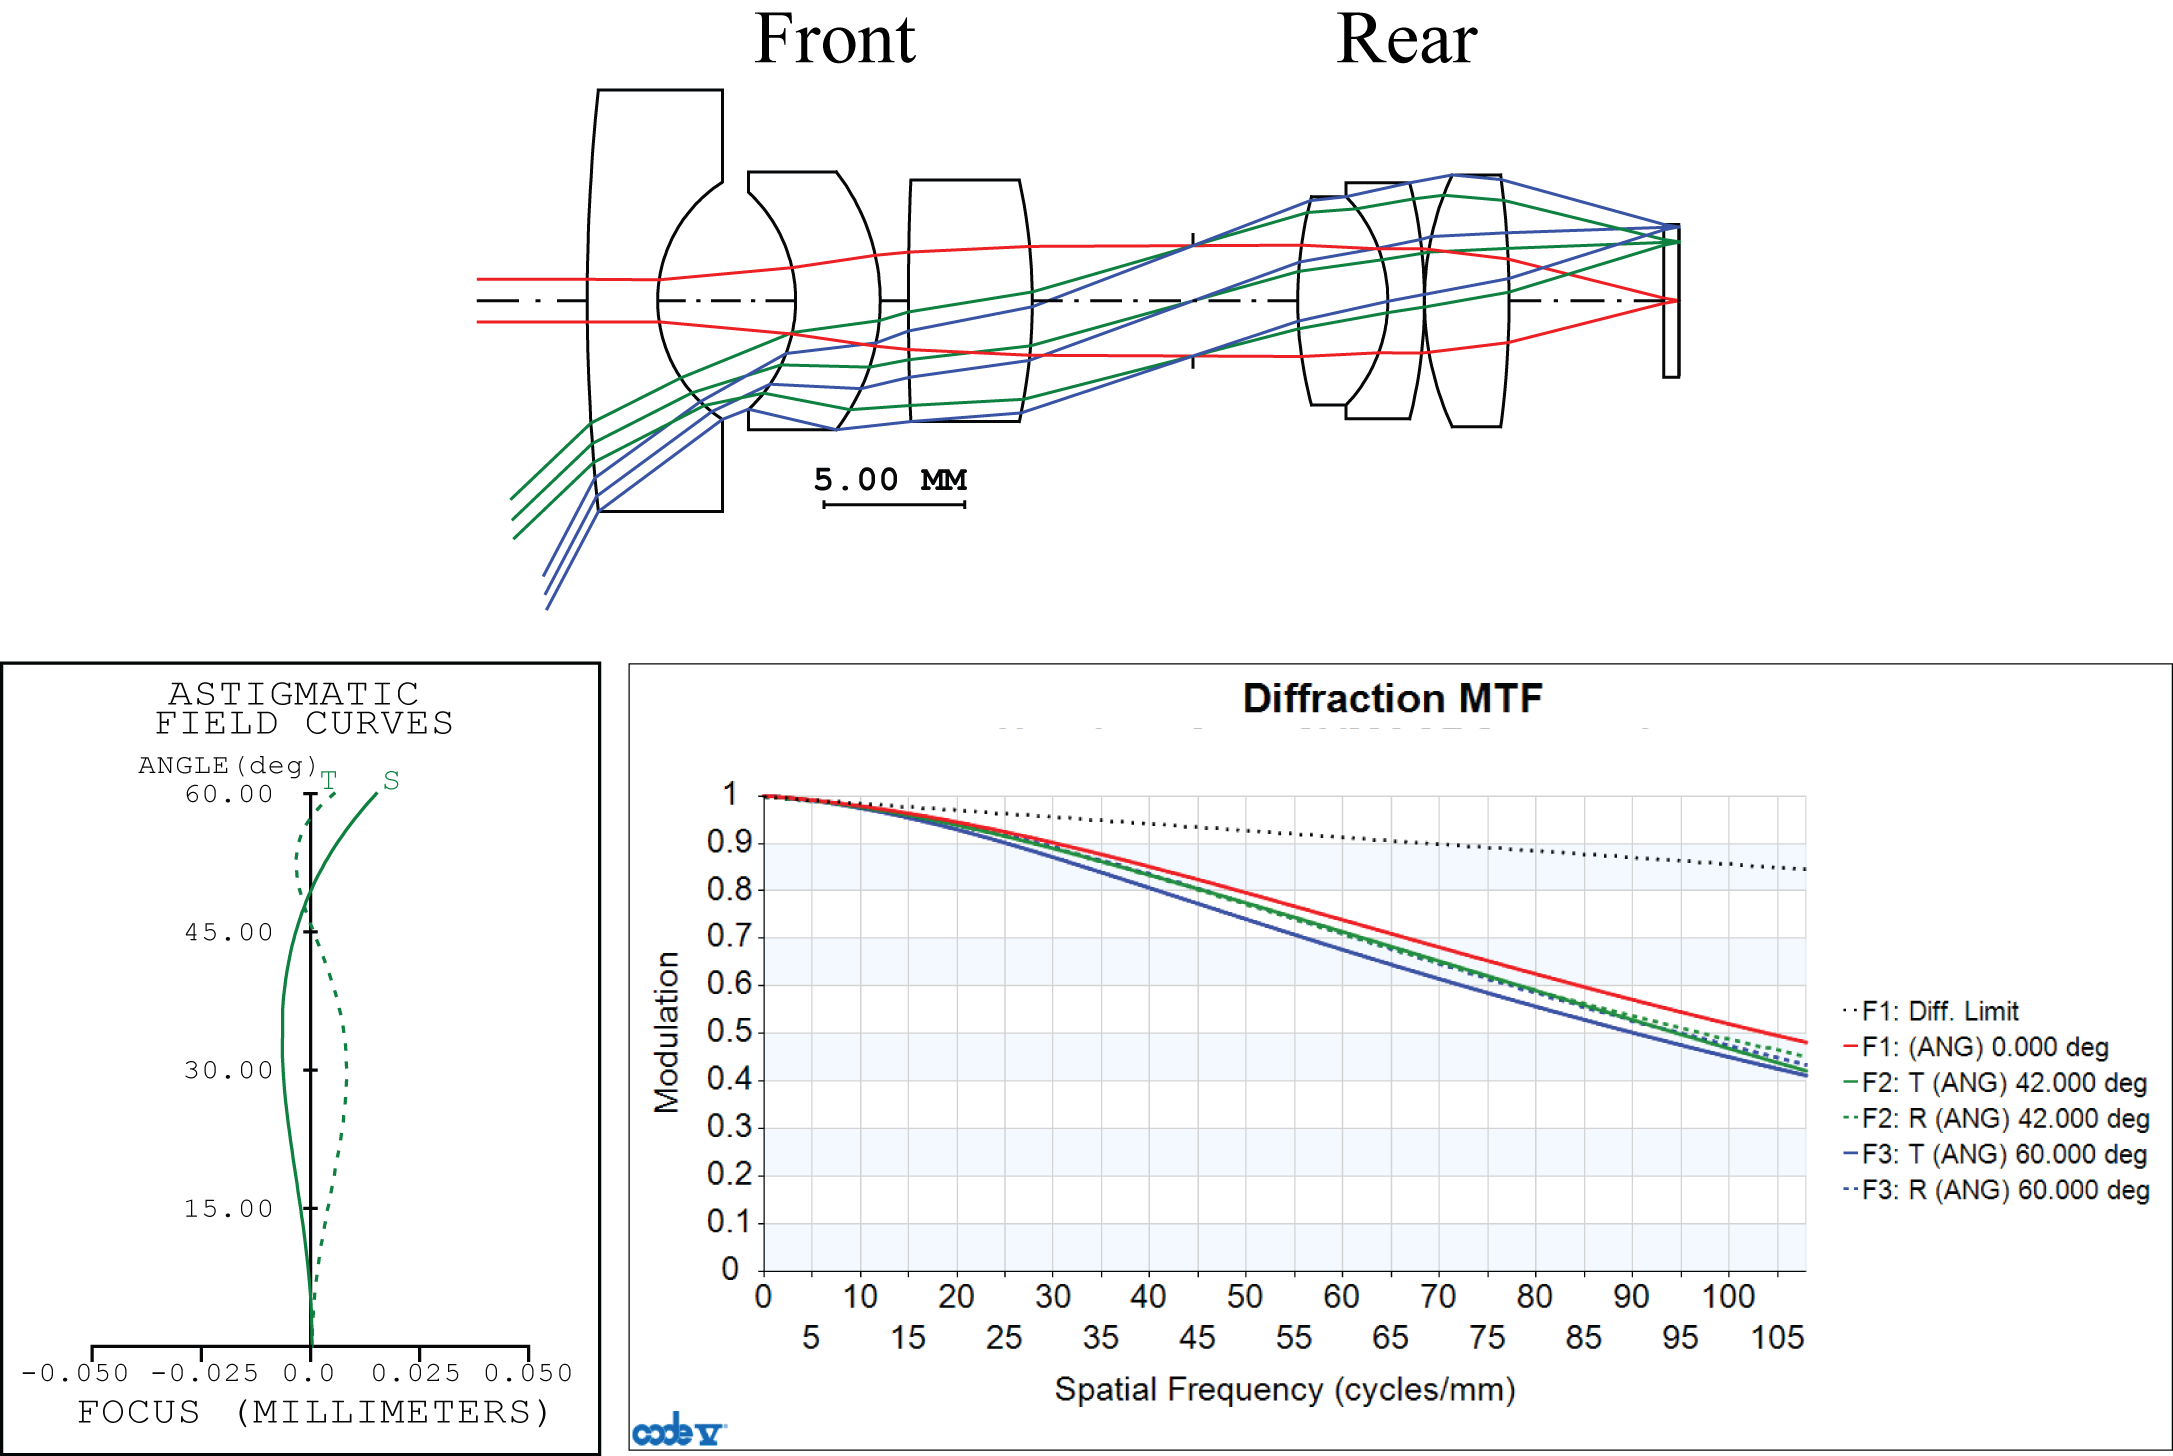
\includegraphics[scale=0.68]{chapter-4/figures/WideAngleL.png}
    \caption{System plot of a wide angle lens and its performance.}
    \label{fig:wideanglelensPerformance}
\end{figure}

With the conventional method, the design of the front group started with a lens using a flat and a concentric surface, given that the stop is at the right side of the lens. A moderate field of view was first used. Then lenses were added with either concentric or aplanatic surfaces. Adjustment and optimization were done to increase the field of view and achieve an angle reduction ratio of 0.3. The rear group was designed starting with a cemented doublet having a flat surface and two concentric surfaces. Another lens was added and a different glass was used to further reduce the aberration. 
After we reach a result with the conventional method, SPC can be used to look for alternative solutions. One way is to apply SPC to both front part and rear part to obtain all the possible solutions for both parts. Then, different combinations can be tested for the whole system. Another way is to directly combine the two groups and perform SPC on the combined system to look for other solutions. We chose to perform SPC only on the rear group, and then combine the rear group solutions with the front group. Afterwards, we performed SPC on the combined systems.
Figure \ref{fig:WAL_combine} shows the solution after combining the front and rear parts. First, there are three different solutions for the rear part after we performed SPC on the last surface. However, after combining and optimizing the combined system, all three combinations converged to one solution as shown on the right side of Figure \ref{fig:WAL_combine}. 

\begin{figure}[h!]
    \centering
    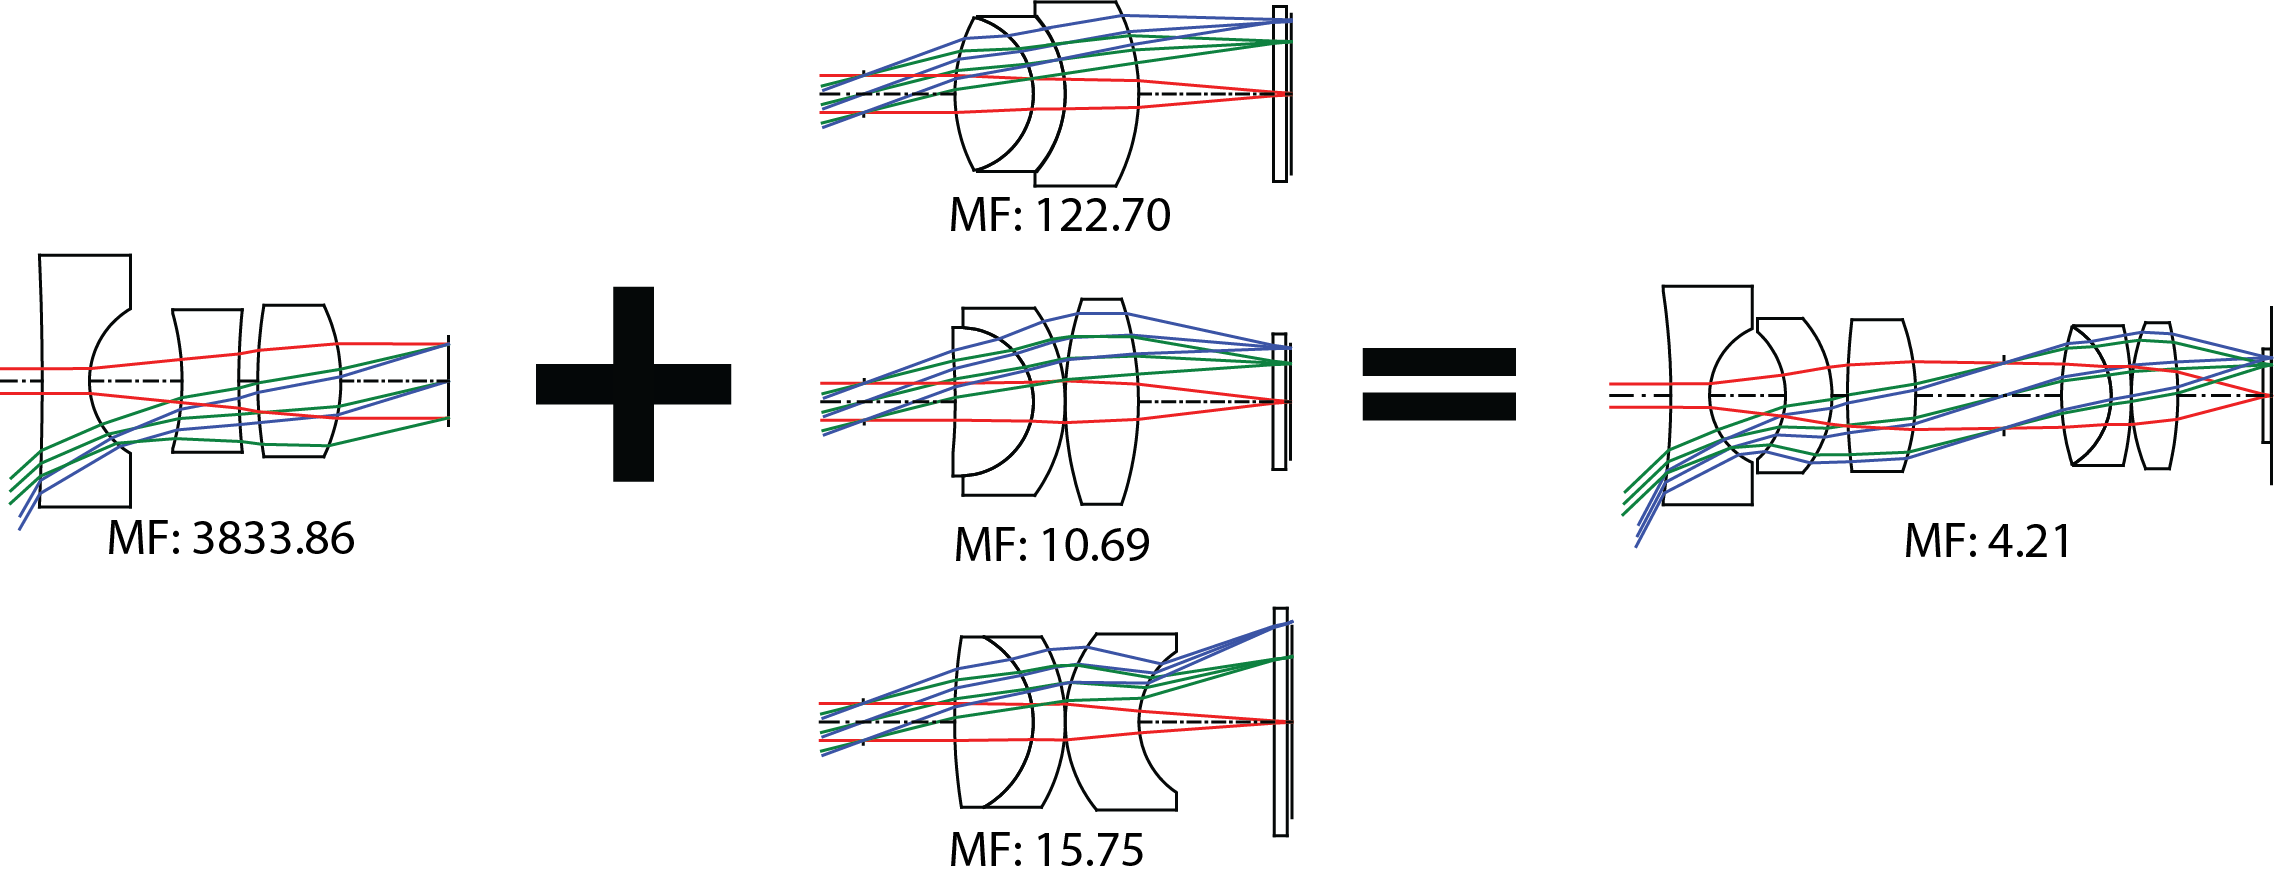
\includegraphics[width=0.7\textwidth]{chapter-4/figures/WAL_combine.png}
    \caption{Combination of the front part and three rear parts all result in one solution.}
    \label{fig:WAL_combine}
\end{figure}

Once the combined system is obtained, we perform saddle point switching in the whole system to look for other minima. Because the first lens is responsible for collecting the large angle rays, extracting it from the system while keeping the large field of view is not possible. Therefore, the possible positions to extract and perform SPC scans are the second, third and last lenses. Six different minima were found in the design network illustrated in Figure \ref{fig:WAL_network}. Global optimization run (Global Synthesis CODE V) was performed, and no new system was found. We notice that the major difference of the systems are in the front group. The lens shape stays the same for the rear group in all six solutions.

The relationship between different systems is indicated by arrows in Figure \ref{fig:WAL_network}. Black arrows show that via SPC, two systems are connected in both ways. For example, by using SPC, M1 can be switched into M2. Starting from M2, SPC reaches M1. Blue arrows indicate a one-way connection. For example, starting from M2, it is possible to find M3 via SPC. However, M3 does not lead to M2. In general, the typical situation is a two-way connection. However, a one-way connection can appear in two situations. In the first situation, a system with high stress and higher value of merit function (MF) is unstable (e.g. M6). It is easy to get out of this kind of poor local minimum with SPC, however, it is not easy (and not necessary for practical purpose) to reach them. The second situation is for two minima which are very close to each other in the design space (e.g. M1 and M2). Systems M1 and M2 that are the best two systems have similar system shapes and close values of MF. Another system obtained by switching from M1, can easily, when switched back, go to M2. However, we see that all minima are connected, which means that starting from any of the minima in the network, there is always a route to reach any other system. It can also be observed that M3 – M6 are all directly connected with the best two systems M1 and M2. This means that if the design process is trapped in one of the poor local minima, applying SPC will switch to one of the best two systems in the network without intermediate steps.  

\begin{figure}[h!]
    \centering
    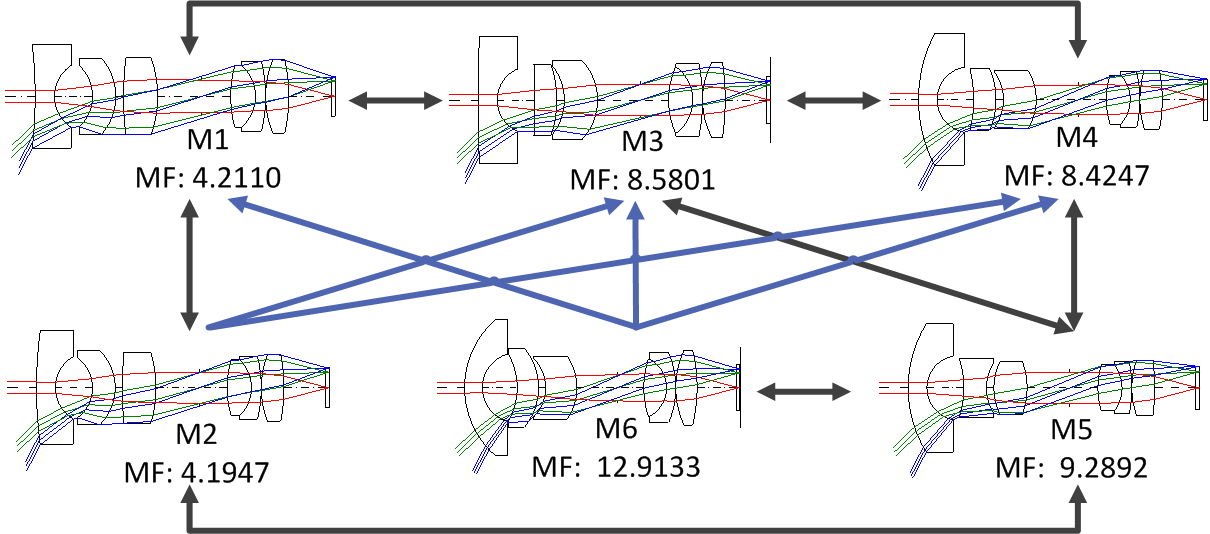
\includegraphics[width=0.8\textwidth]{chapter-4/figures/WAL_network.png}
    \caption{A network of minima for the wide angle lens. All systems are connected with SPC. Global optimization using CODE V did not find extra systems. CODE V transverse ray aberration is used as the merit function.}
    \label{fig:WAL_network}
\end{figure}

\subsection{Analysis of SPC in detailed steps}
The system M3 in Figure \ref{fig:WAL_network} is used as a demonstration to show how SPC is practically performed. First, by extracting the second element from M3, a minimum with one lens less was obtained. Then, an SPC scan was done at the same position where the lens was extracted. Figure \ref{fig:WAL_demo_sp} shows the SPC scan curve and the saddle point system which was found via the scan. In an SPC scan curve, the crossing of the curve and the horizontal axis indicates the curvature of the saddle point system (the black dot in Figure \ref{fig:WAL_demo_sp}). In this case, only one saddle point system is found via the scan and the curvature of the saddle point system is -0.170. By constructing a 2-D plane in the high dimensional space (10-D in this case), it is possible to visualize the saddle point. We already know the value of the merit function at the saddle point, $MF_{S}$, and there exists a direction from the saddle point in which the value of the merit function will decrease. 
\begin{figure}[h!]
    \centering
    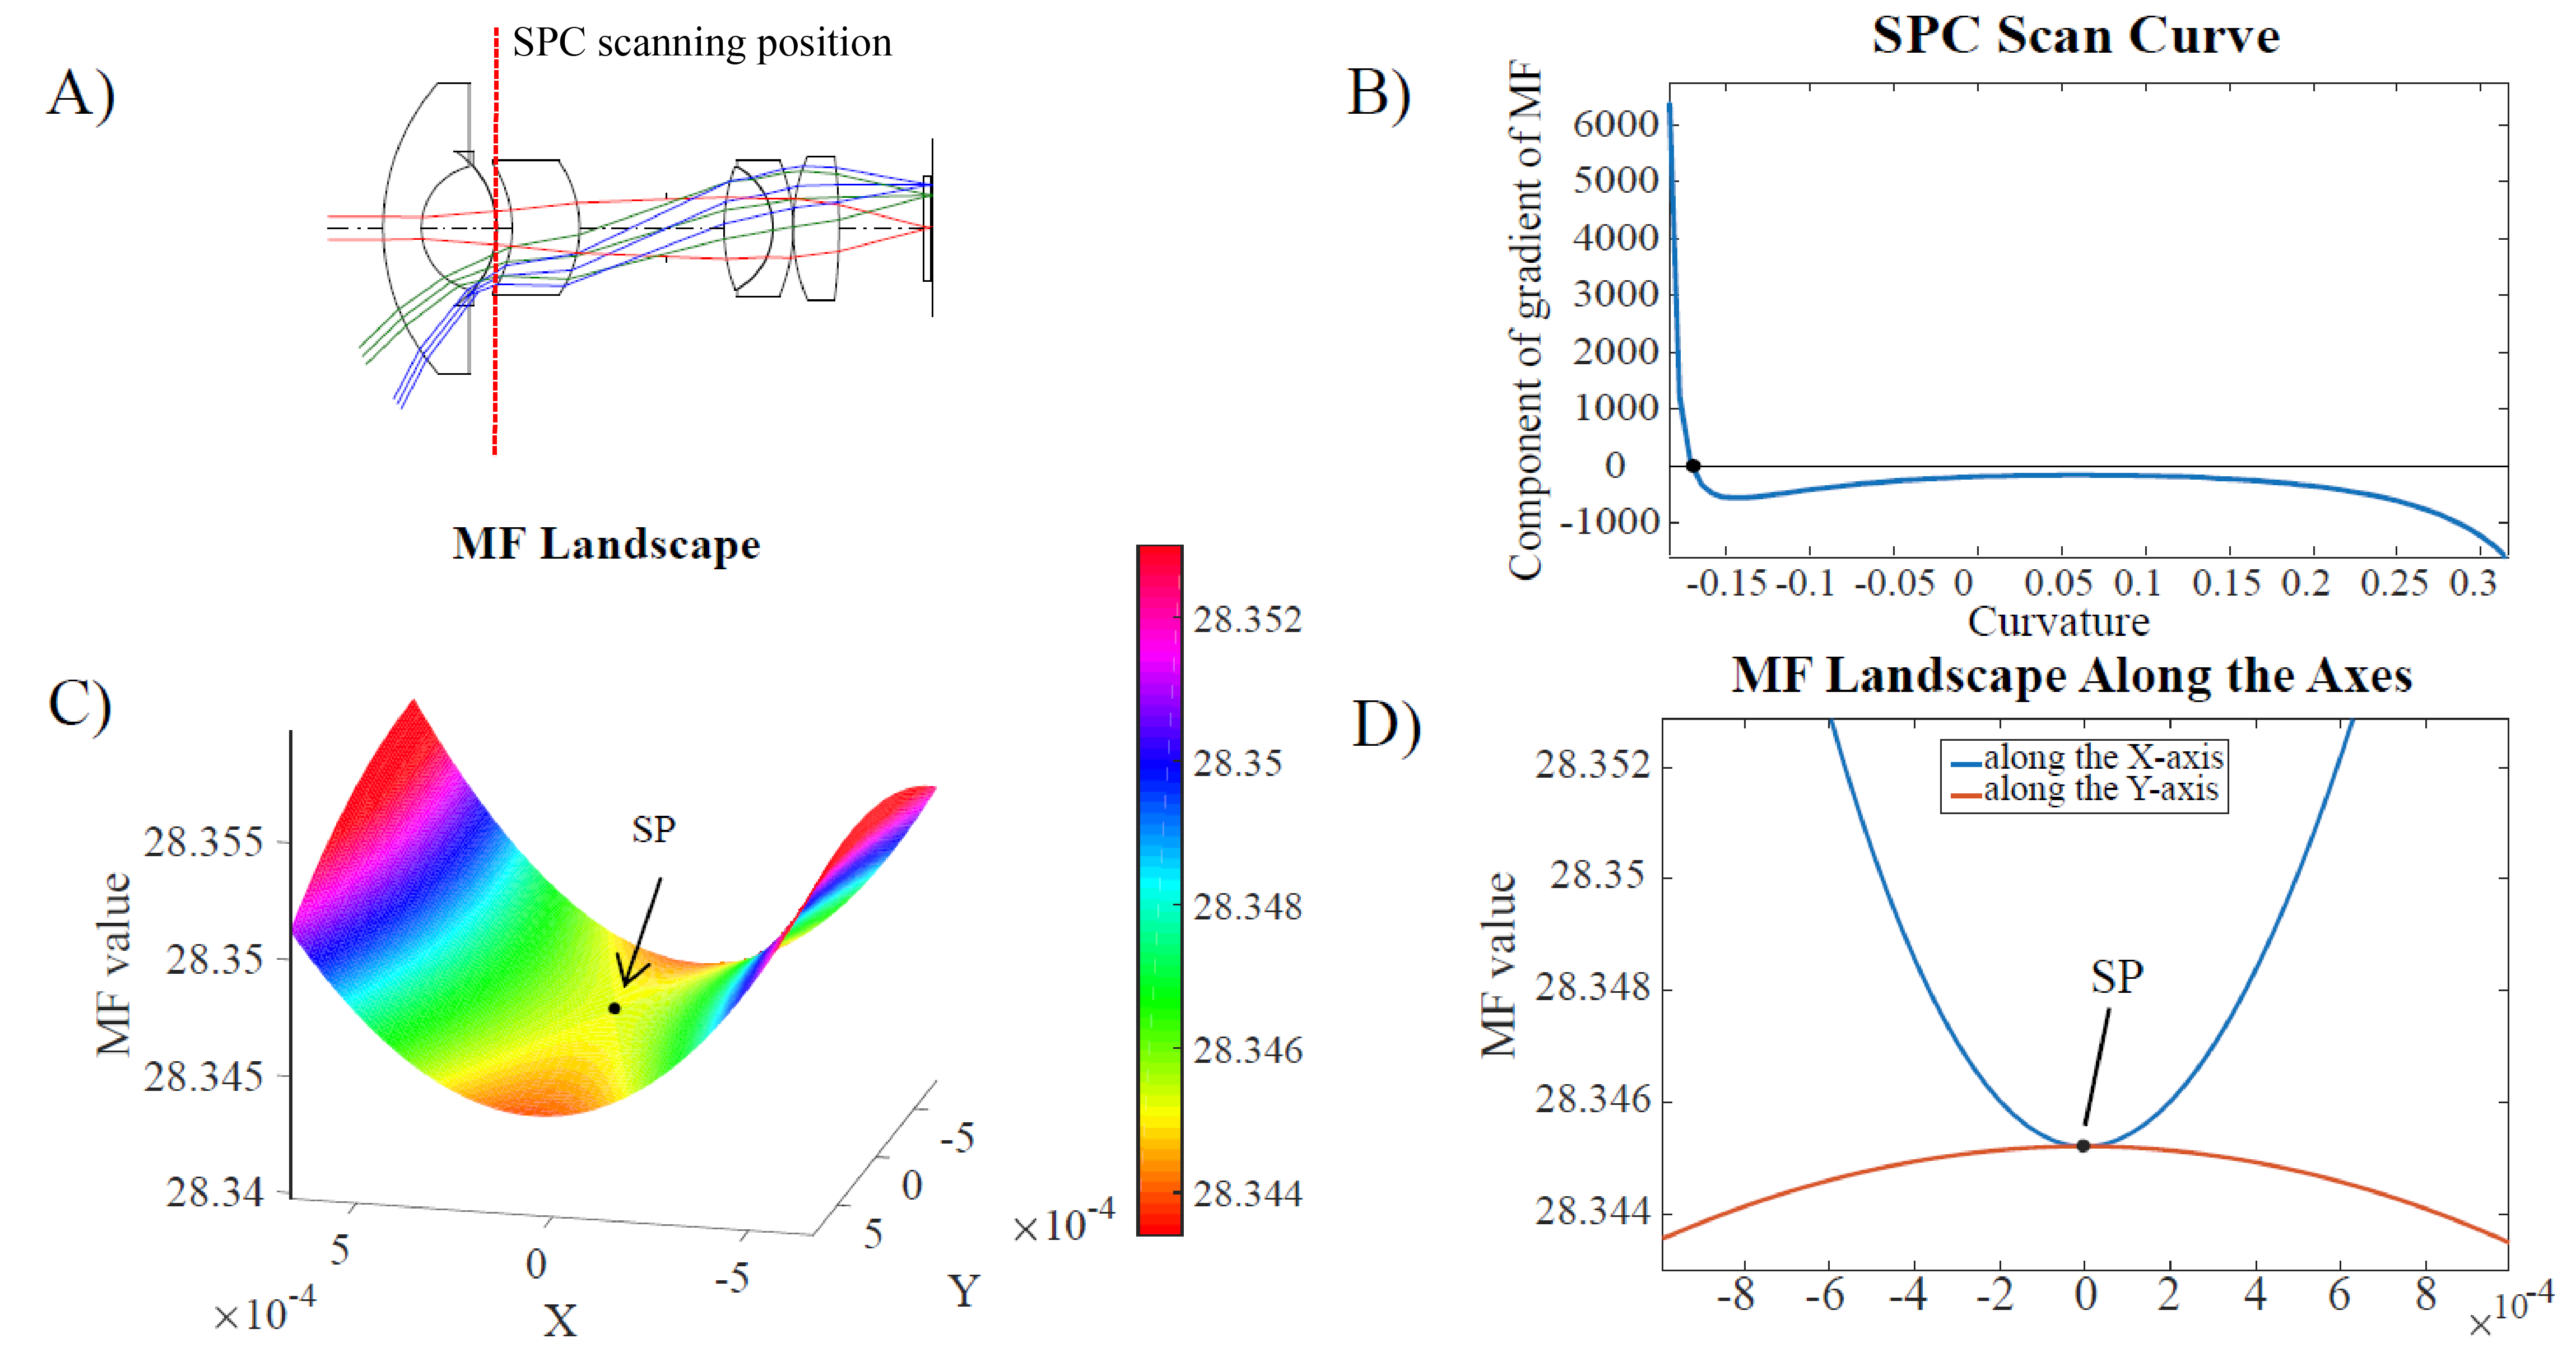
\includegraphics[width=\textwidth]{chapter-4/figures/WAL_demo_sp_2.png}
    \caption{A): the system we have chosen for the SPC scan. B): the SPC scan curve. C): the saddle point in a 2-D plane chosen as shown in the Appendix. D): the descending and ascending direction around the saddle point in the same 2-D plane. The saddle point is marked with a black dot.}
    \label{fig:WAL_demo_sp}
\end{figure}
Numerically, we can find this direction by minimizing on a hyperplane, which is orthogonal to the SPC scan line along which the MF value is constant. As illustrated in Figure \ref{fig:hyperplane}, point $S$ is the saddle point, point $A$ is a point on the equal MF line (where the two curvatures of the inserted element are the same \cite{MVTurnhoutSPC15}). If there are total $N$ variables in the system, $P1$ is an $N-1$ dimensional hyperplane, which is orthogonal to $\overrightarrow{SA}$ and at the same time passing through point $A$. Point $B$ is a point where the MF value is minimized on hyperplane $P1$. As a result, we will have $MF_{B}$ < $MF_{S}$. With points $A$, $B$ and $S$, a 2-D plane $P2$ can be determined in which we can visualize the saddle point. Given the two vectors on the 2-D plane, $\overrightarrow{SA}$ and $\overrightarrow{SB}$, an orthogonal base can be calculated with the Gram-Schmidt process:

\setlength{\belowdisplayshortskip}{5pt}
\setlength{\abovedisplayshortskip}{5pt}
\begin{equation} \label{eq:u1}
\hat{u}_{1} =  \left\| \overrightarrow{SA}-{\frac{\langle \overrightarrow{SA},\overrightarrow{SB}\rangle}{\langle \overrightarrow{SB},\overrightarrow{SB}\rangle}}\overrightarrow{SB} \right\| 
\end{equation}
\setlength{\belowdisplayshortskip}{10pt}
\begin{equation} \label{eq:u2}
\hat{u}_{2} = \left\| \overrightarrow{SB} \right\|
\end{equation}
with $\hat{u}_{1}$ and $\hat{u}_{2}$ , the 2-D plane with the visualized saddle point can be plotted as shown in Figure \ref{fig:WAL_demo_sp}.
In Figure 12, the Y direction is the direction along which the merit function decreases from the saddle point. We see again the numerical instability indicated by the yellow colour in Figure 12. Around the saddle point, the basins of attraction are those for the blue (MF 5.30) and cyan (MF 8.12) minima, that correspond to the red and green region in Figure 10. The way how the basins of attraction are placed in the 2-D plane in Figure 12, shows that the two minima connected by the saddle point are the ones with MF value 5.30 and 8.12 (the red and the green region in Figure 10). The two basins correspond to systems T2-M1 and T2-M4 in Table \ref{table: scanline}.

\begin{figure}[h!]
    \centering
    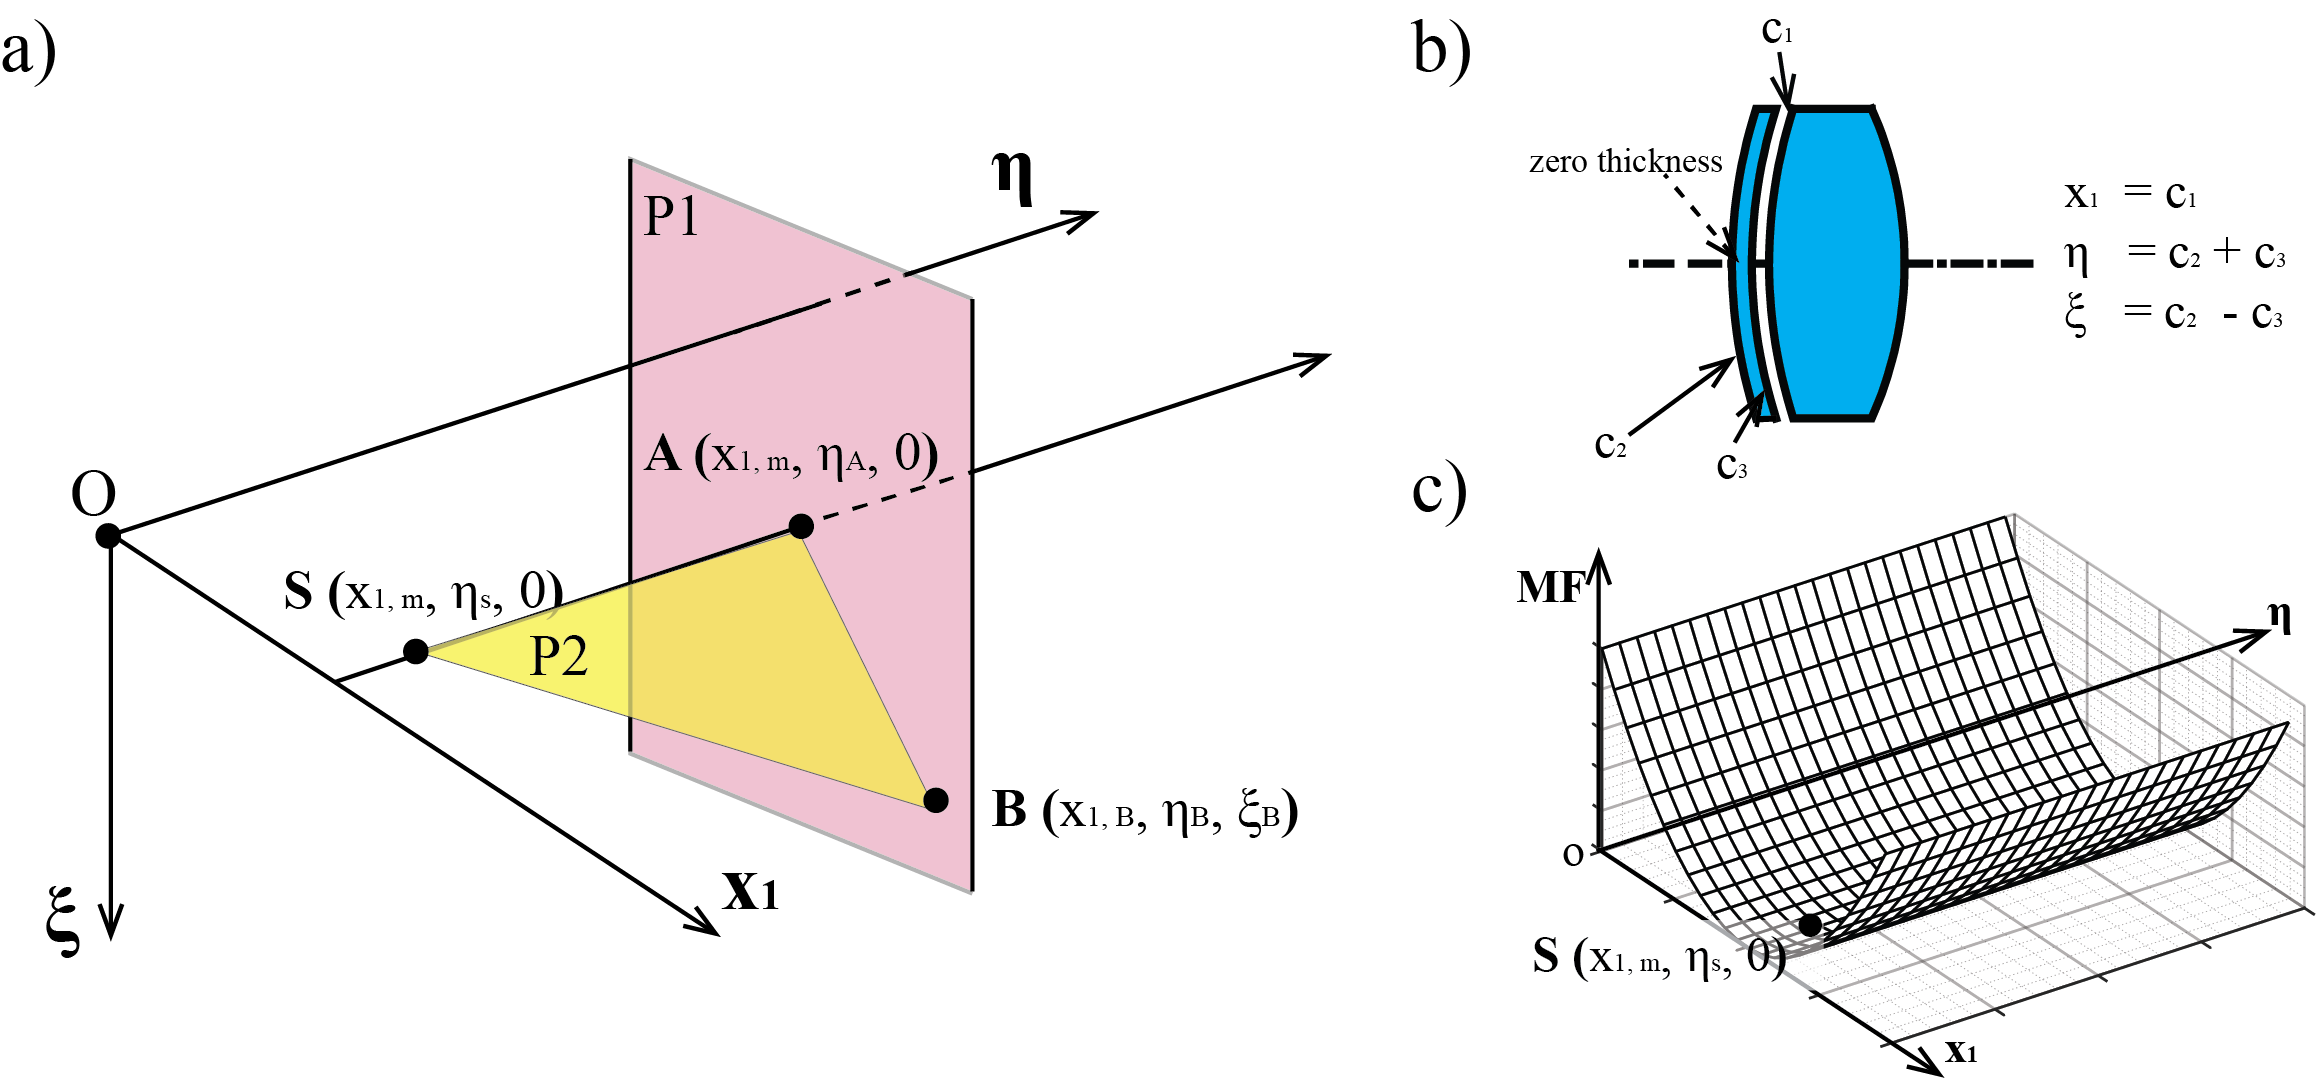
\includegraphics[width=0.65\textwidth]{chapter-4/figures/hyperplane.png}
    \caption{The construction of a 2-D plane(P2) to visualize the saddle point(S). Point A is a point on the SPC scan line. P1 is a hyperplane perpendicular to line SA. Point B is where the MF value is minimized on P1.}
    \label{fig:hyperplane}
\end{figure}
The saddle point in this 2-D plane is illustrated in Figure \ref{fig:WAL_demo_sp}, and the plots along the X and the Y direction show that the value of the MF is increasing in one direction and decreasing in the other direction. Optimization routes following the descending directions on both sides of the saddle (on the Y-axis shown in Figure \ref{fig:WAL_demo_sp}) lead to two distinct local minima.

However, in practice, it is computationally expensive to look for the 2-D plane where the saddle point is visualized as in Figure \ref{fig:WAL_demo_sp}. As mentioned previously, a common practice is to change the system along the SPC scan line, which means changing the curvatures of the inserted null-element with a small positive and negative value (this value is chosen empirically). The modified systems are the starting points for optimization. However, choosing different values for the curvature change may lead to different minima. This is demonstrated in Figure \ref{fig: scanning_line}, where we have chosen different values for the null-element curvature as a starting point and optimize to a minimum. In order to better illustrate the phenomenon, the scan range chosen here (from -0.2 to 0.2) was larger than the curvature changes we normally use in practices for SPC. From Figure \ref{fig: scanning_line}, we see that five different minima were obtained with different values chosen for the start curvature. The system shapes and MF value are shown in Table \ref{table: scanline}. 
\begin{table}[h!]
    \centering
    \captionsetup{justification=centering}
    \caption{Result of the optimization along the scan line}
    \label{table: scanline}
    \vspace{-1em}
    \hspace*{-16.5pt} %adjusting the position of the plot(table)
    \begin{tabular}{l}
    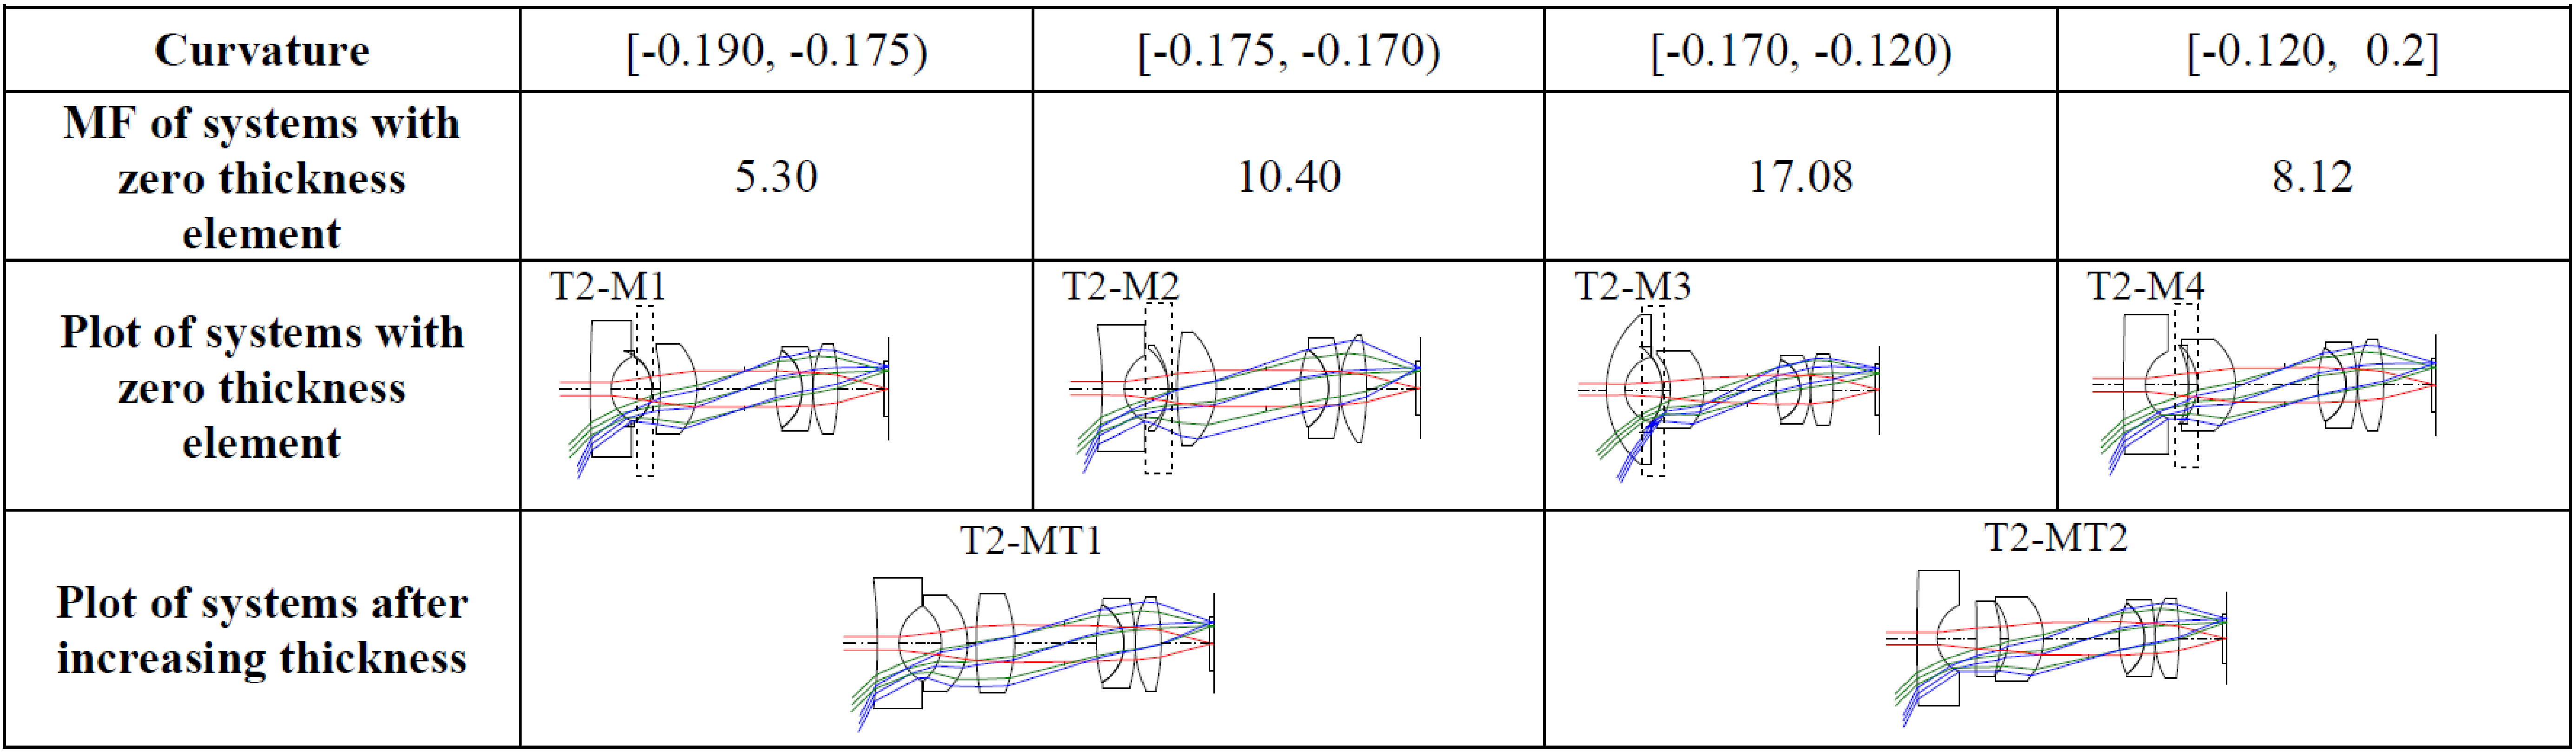
\includegraphics[width=0.98\textwidth]{chapter-4/figures/Line_Opt_table.png}
    \end{tabular}
\end{table}
\begin{figure}[h!]
    \centering
    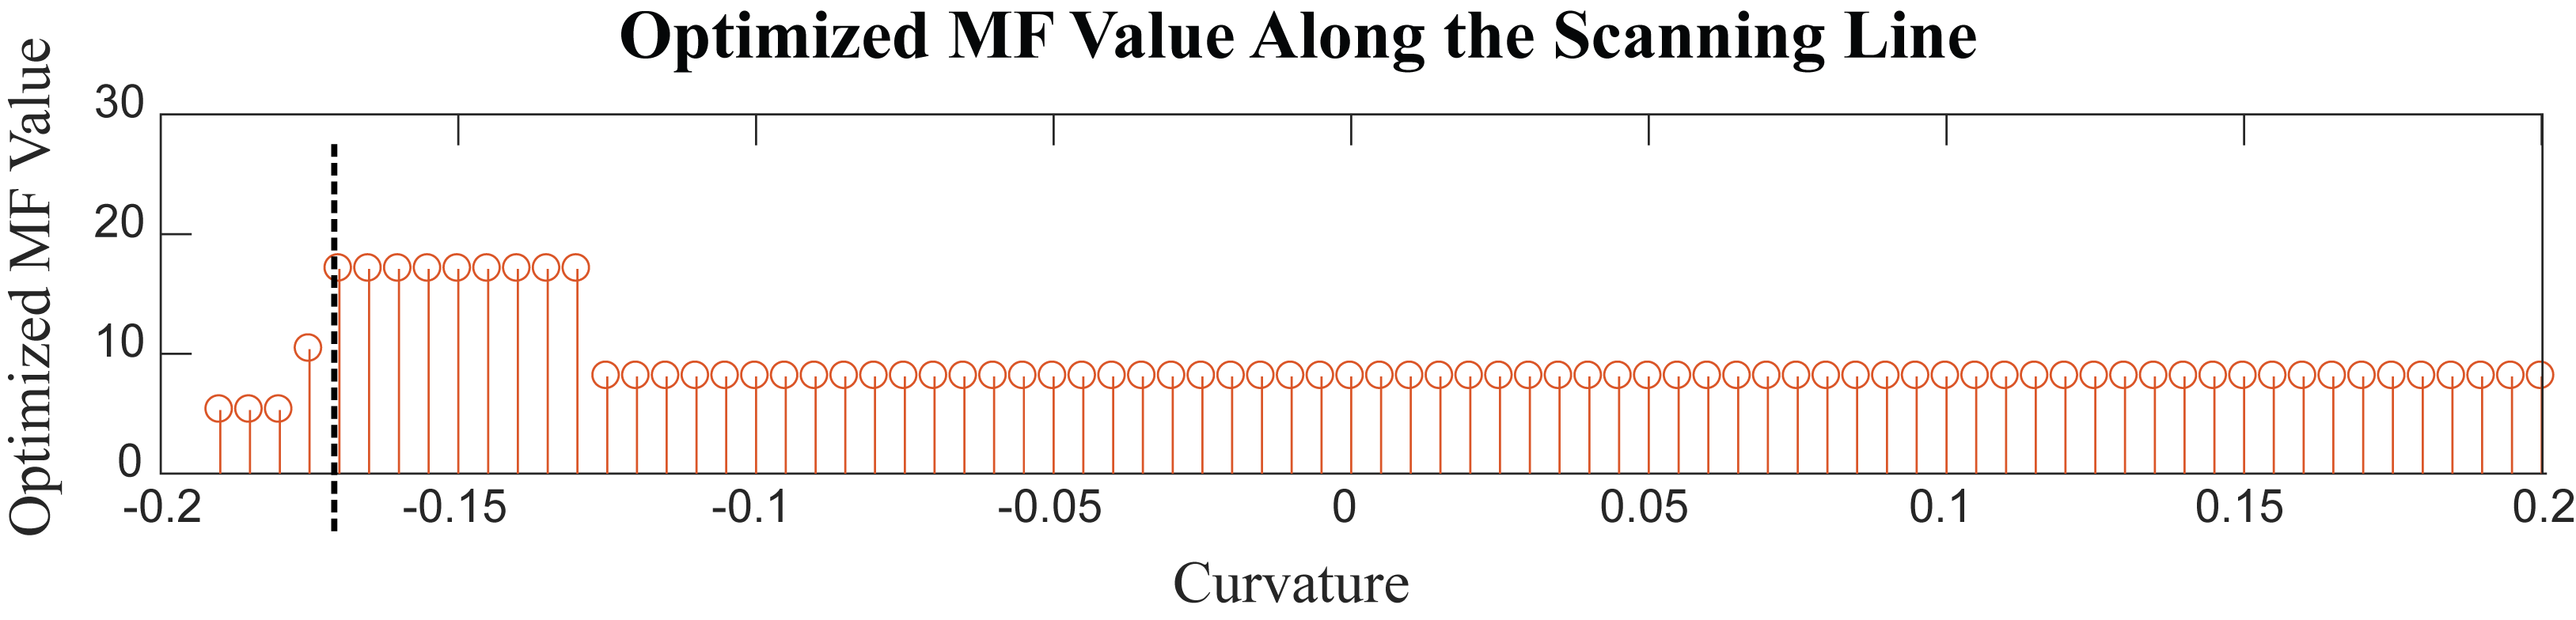
\includegraphics[width=0.95\textwidth]{chapter-4/figures/Scanning_Line_plot.png}
    \caption{Optimized MF value along the scan line. The vertical dashed line indicates the saddle point curvature.}
    \label{fig: scanning_line}
\end{figure}
It is also possible to choose the starting points on a 2-D plane, where the saddle point locates. We plot the optimization results on two of these 2-D planes to compare: one is the plane determined by equation \ref{eq:u1} and \ref{eq:u2}; the other is the plane determined by the two newly inserted variables. As shown in Figure \ref{fig:basins}, the right side of the plot show the basins of attraction in a large region, from which the complexity of the optimization landscape can be observed. On the right side of the plot, the local region around the saddle point is plotted. In both plots, the scan line divides the basins into two parts: the green part converging to the minimum with a MF value of 8.12 and the red part converging to the minimum with a MF value of 5.30. In both cases, we also observe that if the starting points are chosen on the scan line, the optimization may converge to the minimum with a MF value of 17.08 (yellow color) or the minimum with a MF value of 10.40 (navy blue color). Shown by the consistent results from both plots, the red and green regions represent the two basins on both side of the saddle point. However, in this case, choosing starting points on the scan line may lead to unwanted local minima. Practically, it is still recommended to choose the starting points on the inserted 2-D plane since it does not involve extra computation. From the plots in Figure \ref{fig:basins}, it shows that a better to choose the starting points is to avoid the scan line, for example, perpendicular to the scan line. It is also seen that the starting points should not be too far away from the saddle point. Otherwise, the two basins around the saddle point will be missed. In Figure \ref{fig:basins} (B, the saddle point has its coordinates of $(-0.1702,-0.1702)$. The closest point where the optimization converges to unwanted minimum is $(-0.1713, -0.1675)$. The distance between to two points is $0.0029$, which is $1.7\%$ of the absolute value of the curvature at the saddle point. 
\begin{figure}[h!]
    \centering
    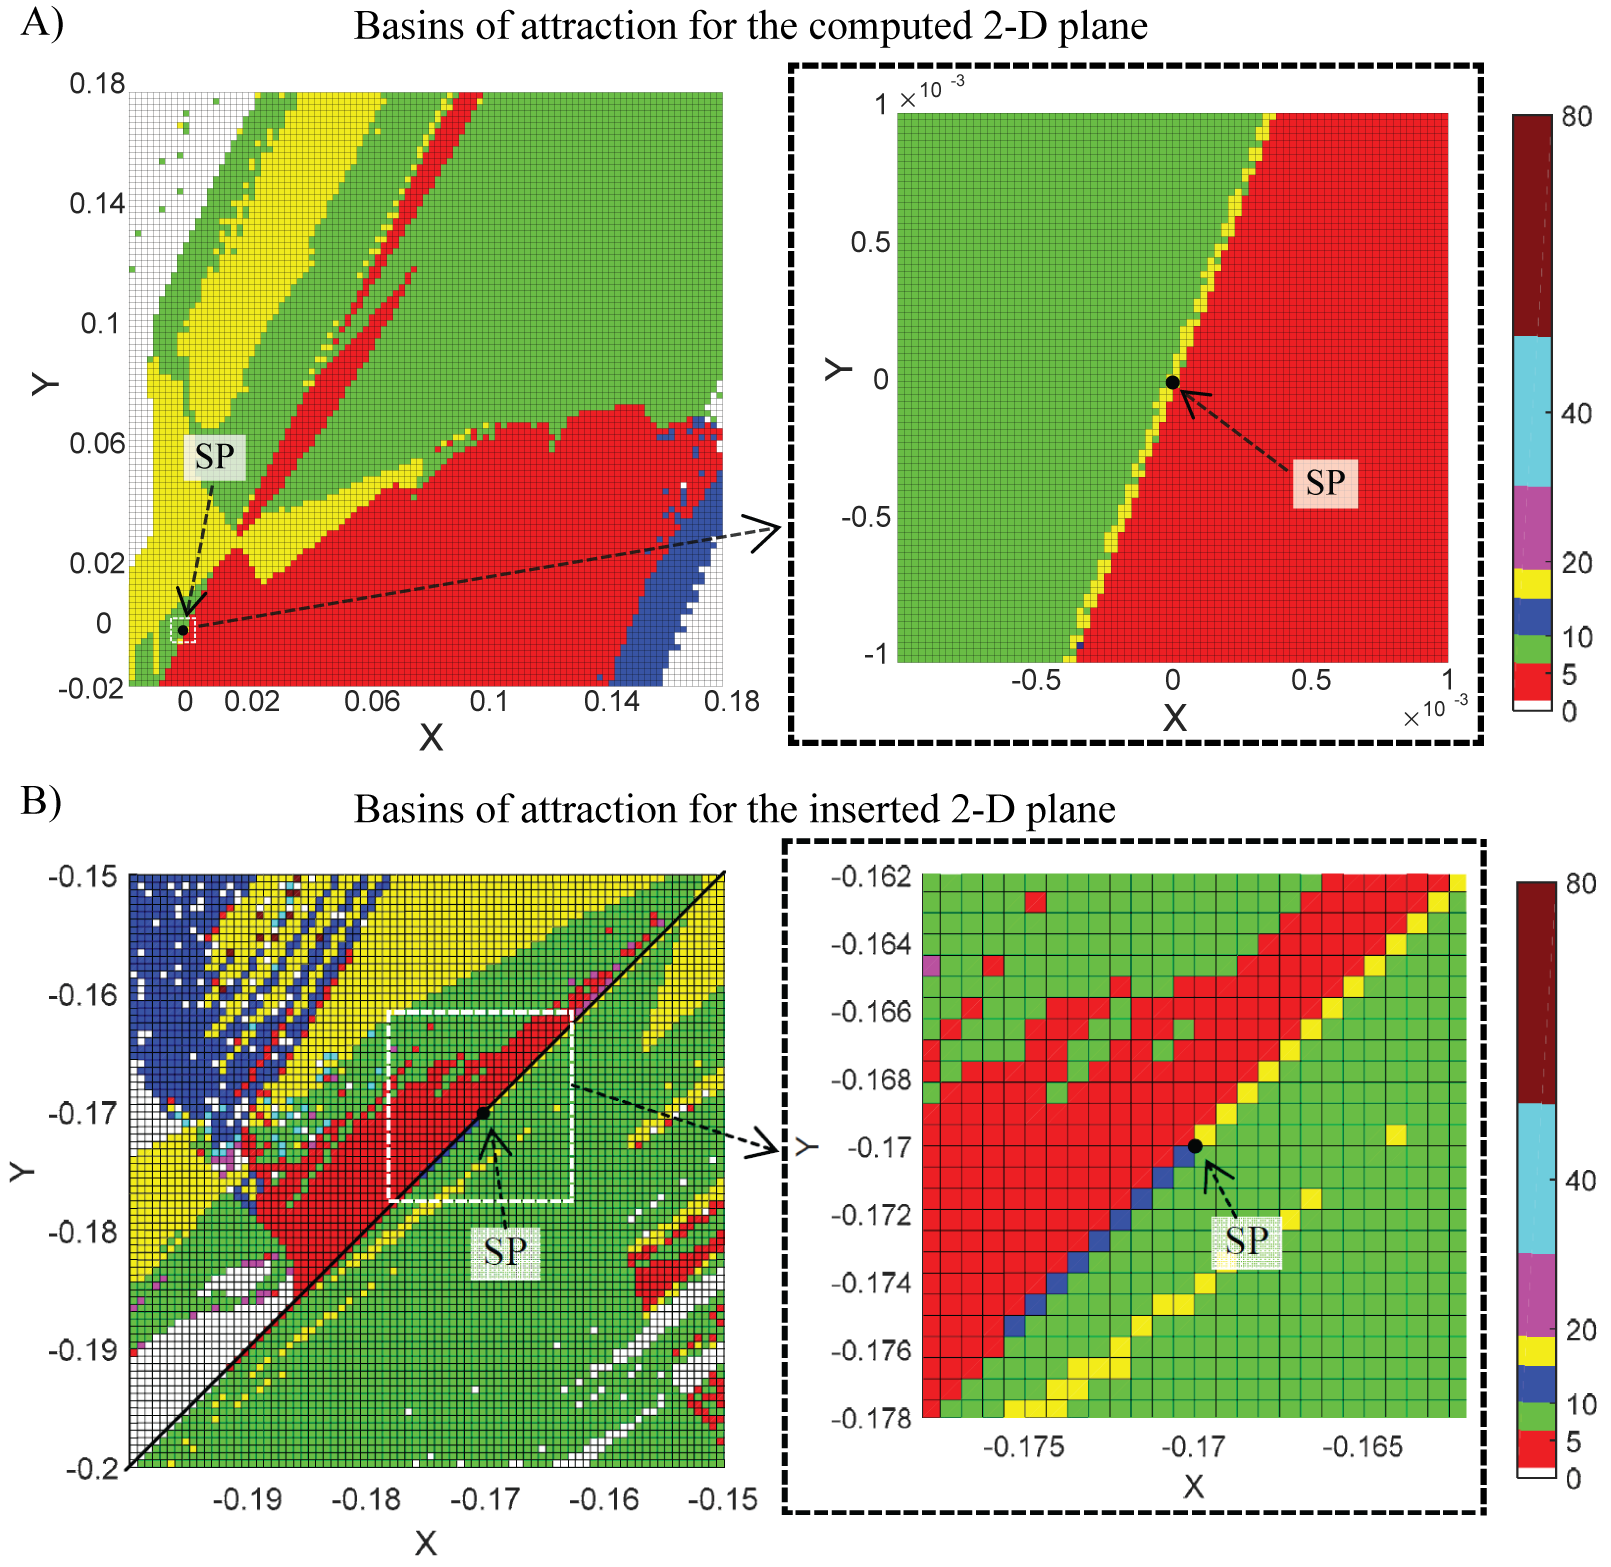
\includegraphics[width=0.8\textwidth]{chapter-4/figures/Basins_two_situations.png}
    \caption{Basins of attraction around the saddle point in 2-D planes. A) Computed 2-D plane given by equation \ref{eq:u1} and \ref{eq:u2}; B) 2-D plane given by the two newly inserted variables. The saddle points (SP) are marked by black dots.}
    \label{fig:basins}
\end{figure}
It is not clear yet why on the scan line the optimization shows such a behavior. It has been demonstrated in \cite{vanTurnhoutThesis2009} (Page 81) that when the damping factor of the damped least square algorithm is sufficient, there will be less artifacts shown in the plot of the basins of attraction. On the scan line, there is no artifact that lead to a different local minimum. Since we do not have control of the damping factor in CODE V, we cannot test whether it is caused by the choice of damping factor. Nevertheless, it is possible to look at the basins of attraction plot in a different scanning position. We extracted the third lens and chose to scan for saddle point at that position. As shown in Figure \ref{fig:basins_WAL_M3_S5}, along the scan line, there are no artifacts that lead to a different local minimum. In this case, choosing starting points along the scan line at different sides of the saddle point will lead to different local minima. It will either converge to the green region (MF = 44.53) or the orange region (MF = 37.82). White region (MF = 0) indicates ray failure. The closest starting point, which the system can still be ray traced, is at $(-0.1893, -0.1960)$. The coordinates of the saddle point is $(-0.1903, -0.1903)$. The distance between them is $0.0058$, which is $3.0\%$ of the absolute value of the curvature of the saddle point. 
\begin{figure}[h!]
    \centering
    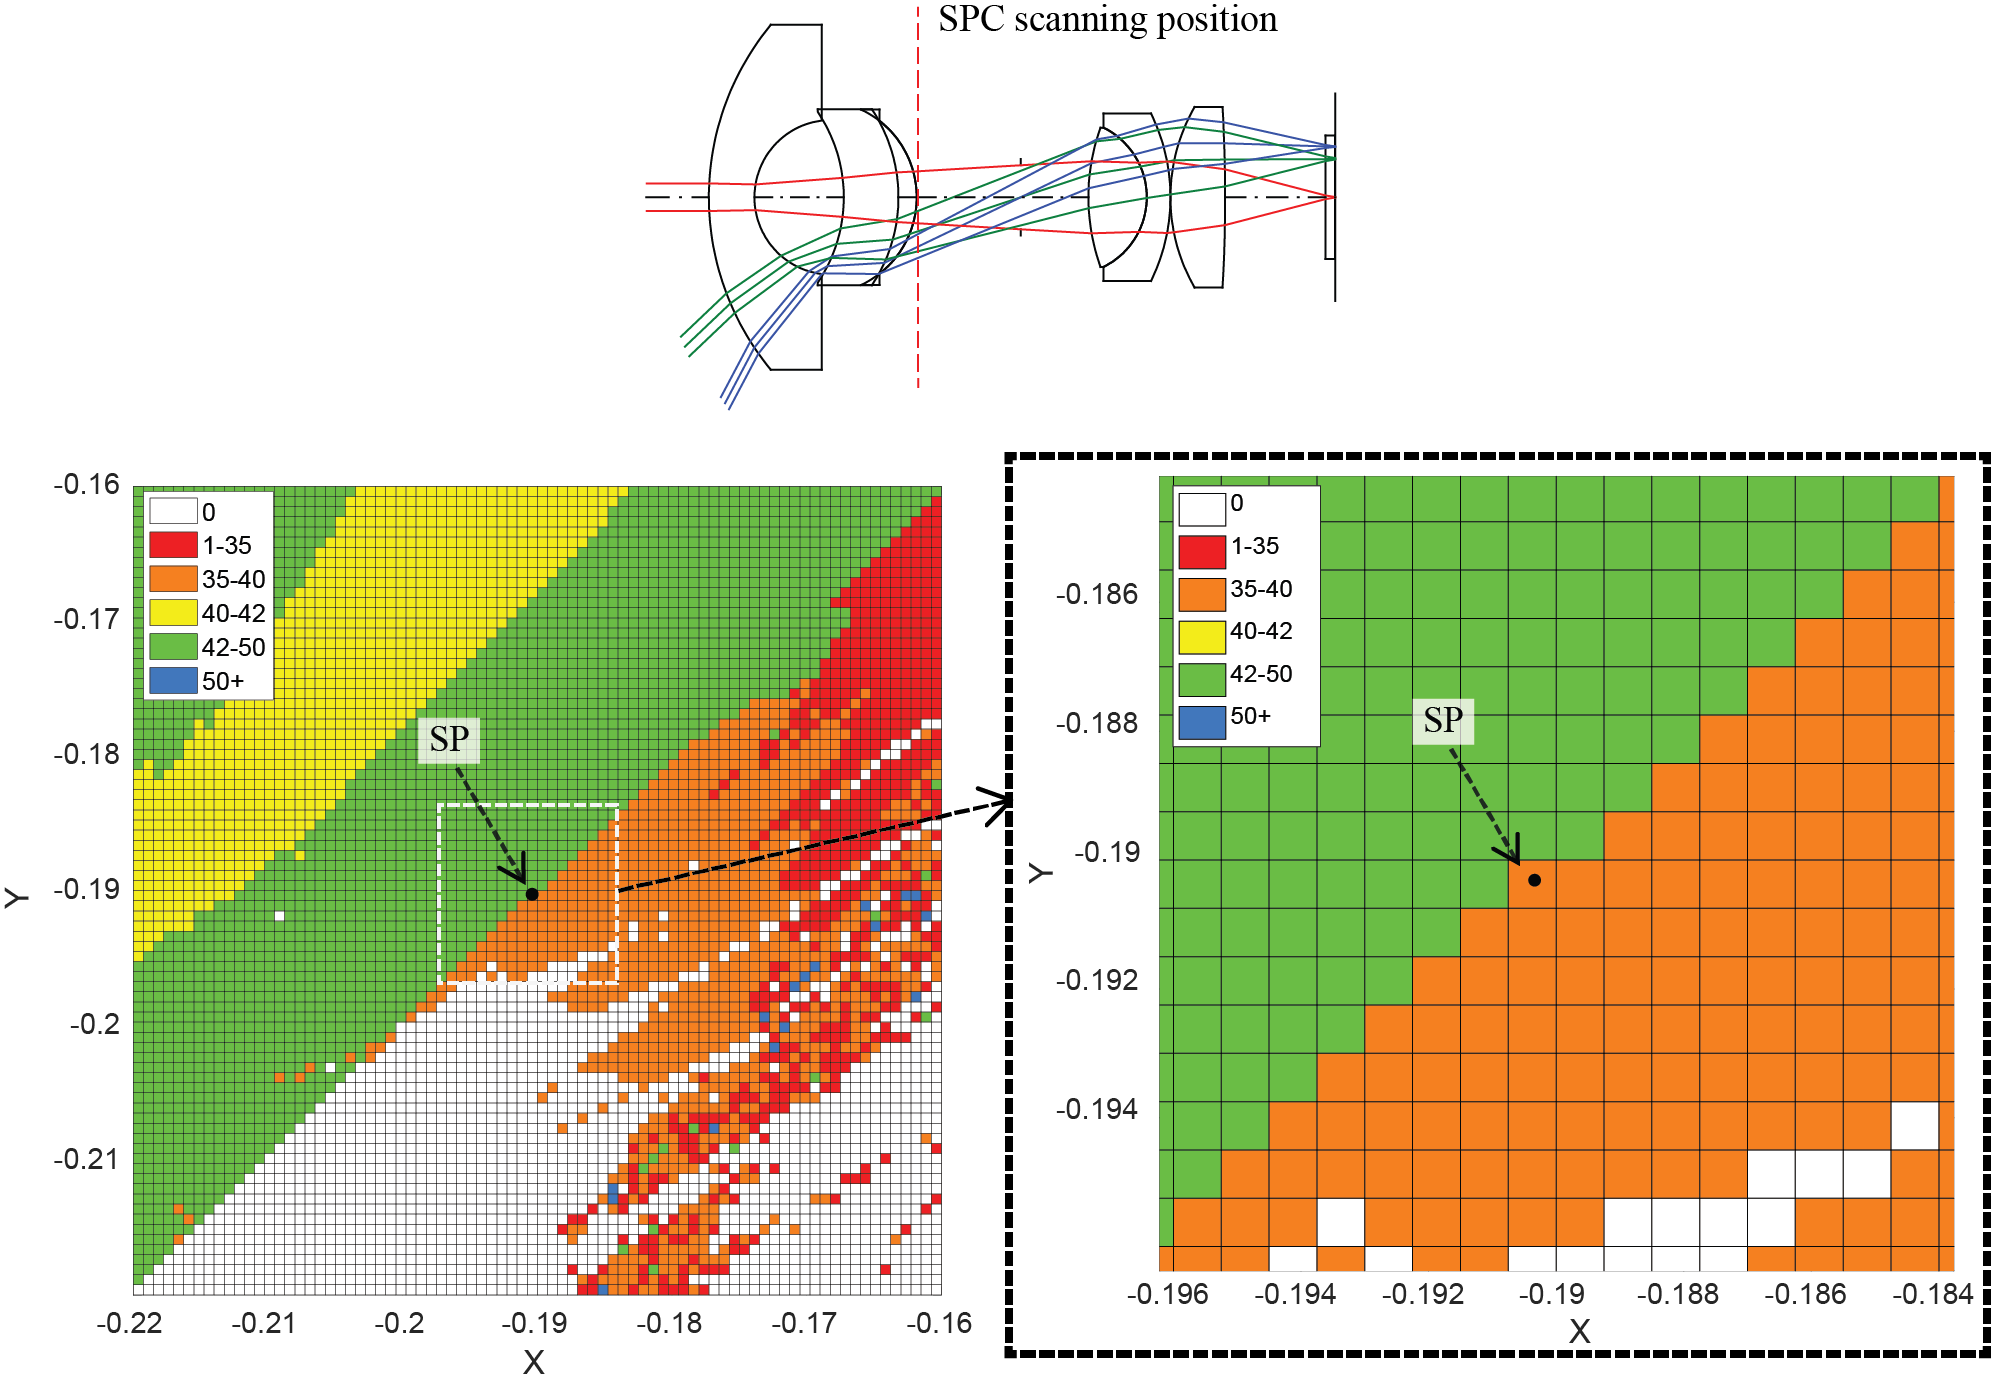
\includegraphics[width=0.8\textwidth]{chapter-4/figures/M3-S5_basins.png}
    \caption{Basins of attraction at a different scanning position compared to \ref{fig:basins}. Along the scan line (diagonal line in the plot) around the saddle point, there are no artifacts that lead optimization to minima other than the two near the saddle point.}
    \label{fig:basins_WAL_M3_S5}
\end{figure}
To obtain minima that are practical, the zero thickness of the inserted element will be increased, as shown in the bottom row of Table \ref{table: scanline}. The two minima on the left side of the saddle point (T2-M1 and T2-M2) converged to minimum T2-MT1, and the two minima on the right side of the saddle point (T2-M3 and T2-M4) converged to minimum T2-MT2. When the thickness was increased, T2-M2 and T2-M3 merged with T2-M1 and T2-M4 respectively. This is shown by plotting the optimized value of MF while increasing the thickness in small steps (Figure \ref{fig:thickness_increase}). In Figure \ref{fig:thickness_increase}, the curve of T2-M3 has a jump around thickness 2 mm where the MF value suddenly changed. Before the changing point, the system became very stressed as shown in the figure. A slight change of thickness made system T2-M3 merged with T2-M4. The curve of T2-M4 stays smooth indicating that this minimum is a stable minimum while changing the thickness. The same situation happened with T2-M2: it merged with T2-M1 right after increasing the thickness. A detailed analysis using basins of attraction near the saddle point (Figure \ref{fig:basins}) shows that the stable minima T2-M1 and T2-M4 are the two zero-thickness minima connected by the saddle point.
 In this example,  we have seen that choosing different distances from the saddle point along the scan line can lead to more than two minima after the first optimization from the SP system in Figure \ref{fig:WAL_demo_sp}. Even though this is not always the case, we suggest that a starting point should be chosen outside the scan line to prevent trapping in unwanted local minima. Data shown that the starting points can be chosen within a distance from the saddle point of $2.4\%$ of the absolute value of the saddle point curvature. Experiment results show that often many zero-thickness minima obtained in the intermediate steps of SPC are not stable and disappear after increasing the thickness of the new element. Therefore, the final result (two finite-thickness minima on both sides of the saddle in this example) is typically less dependent on the precise choice of the perturbation curvature.  
\begin{figure}[h!]
    \centering
    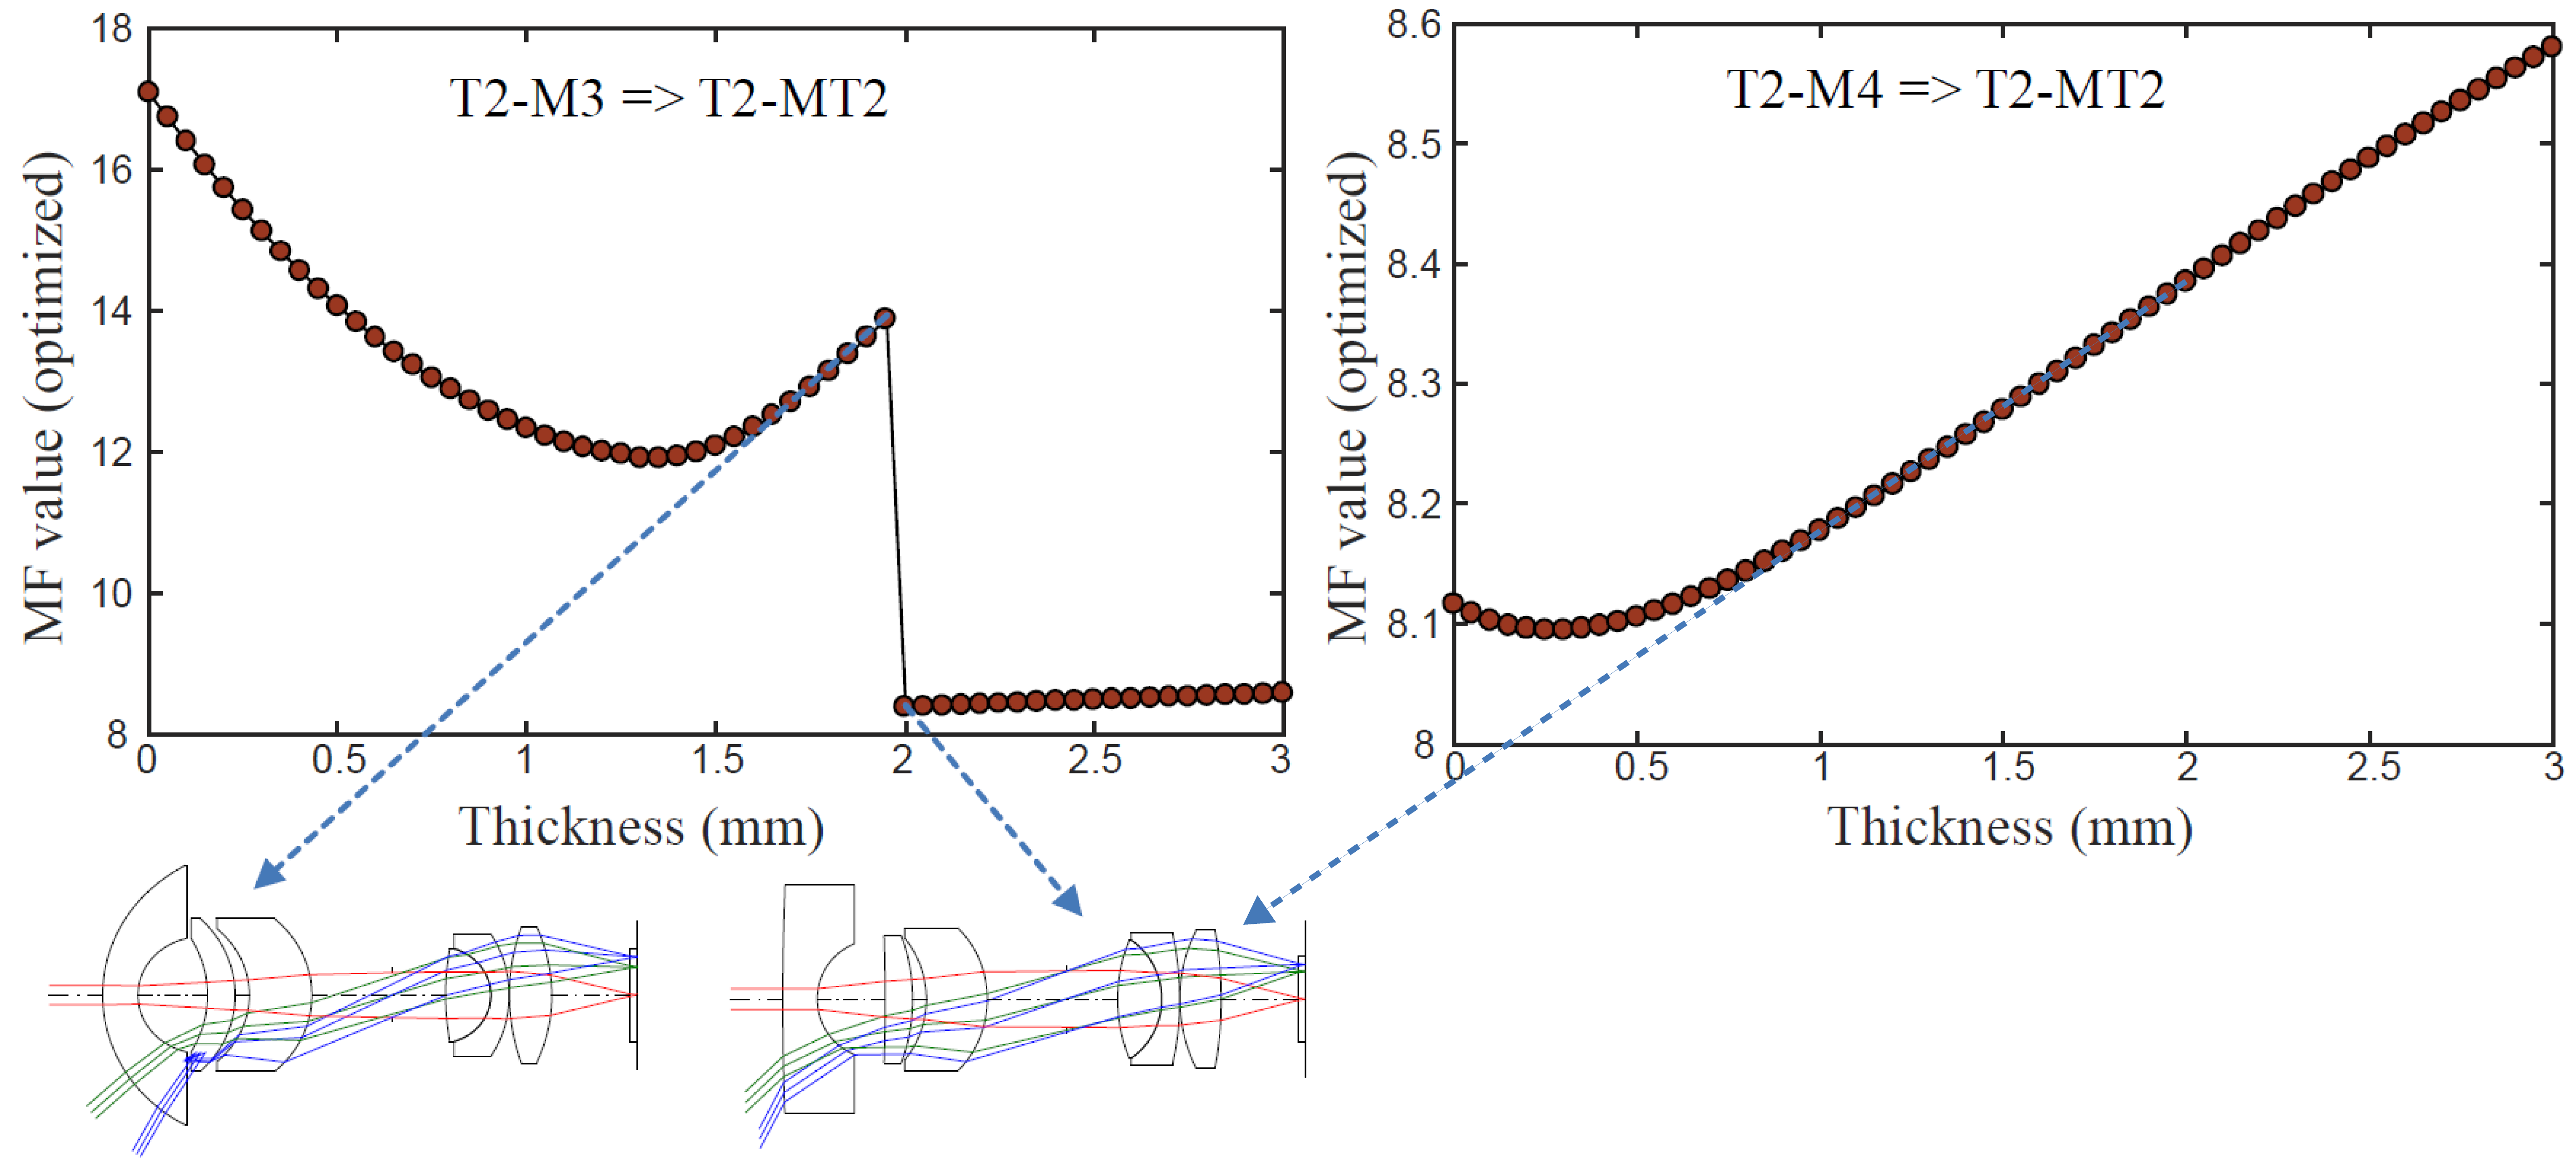
\includegraphics[width=0.8\textwidth]{chapter-4/figures/thickness_increase.png}
    \caption{Change of the optimized value of the merit function while increasing the thickness of the zero-thickness element. T2-M3 and T2-M4 correspond to systems when the thickness is zero. T2-MT2 corresponds to the system when the thickness equals to 3 mm. The discontinuity of the left plot indicates the instability around a minimum in the design space. Systems like the left one are usually poor local minima.}
    \label{fig:thickness_increase}
\end{figure}

\section{Applying SPC to a microscope objective}
\subsection{Ultraviolet (UV) microscope dry objective}
Working together with a designer in Jena, we have chosen a UV microscope objective and applied saddle point construction in practical design cases. The microscope objective is designed by Vollrath and its specification is reported in a published patent \cite{patentvollrath}. One variation from the patent is reproduced in CODE V. The operating wavelength of the system is at 325 nm. The system consists of seven lens elements. The material used in CODE V is fused silica (LithosilQ from SHOTT) with a refractive index of 1.4816 at 325 nm. Specification and performance of the system is listed in Table \ref{table: vollrathspec}. With a barrel lens having a focal length of 250 mm, the magnification of the composite microscope becomes 100. The seven lens elements in the system can be divided into three function groups according to Zhang and Gross \cite{ZhangMicroscope2017}. As shown in the system plot in Figure \ref{fig: vollrathoriginal}, the first lens on the left forms the rear group. The second and third lenses form the middle group, and the rest of the lens elements form the front group. Zhang and Gross categorize the existing microscopes into three types depending on the functions performed by different groups. The distribution of the spherical aberration in different groups shown in Figure \ref{fig: vollrathoriginal} indicates that the middle and rear group correct the spherical aberration together. 

\setlength{\arrayrulewidth}{.5mm}
\setlength{\tabcolsep}{18pt}
\renewcommand{\arraystretch}{1.2}
\begin{table}[h!]
    \centering
    \captionsetup{justification=centering}
    \caption{System specification and performance of the microscope objective}
    \label{table: vollrathspec}
    \vspace{-1em}
    \begin{tabular}{ p{15em}  c }
    \hline 
    Effective focal length (EFL, mm) & 2.5\\ 
    Field (real image height, mm) & 0.1\\ 
    Numerical aperture (NA) & 0.90\\ 
    Operating wavelength (nm) & 325\\ 
    Working distance (WD, mm) & 0.6\\ 
    Overall length (mm) & 25\\
    \midrule
    RMS wave front error (m$\lambda$) & 48.5\\ 
    Strehl ratio at 0 mm & 0.976\\ 
    Strehl ratio at 0.1mm & 0.849\\
    \hline
    \end{tabular}
\end{table}

\begin{figure}[h!]
    \centering
    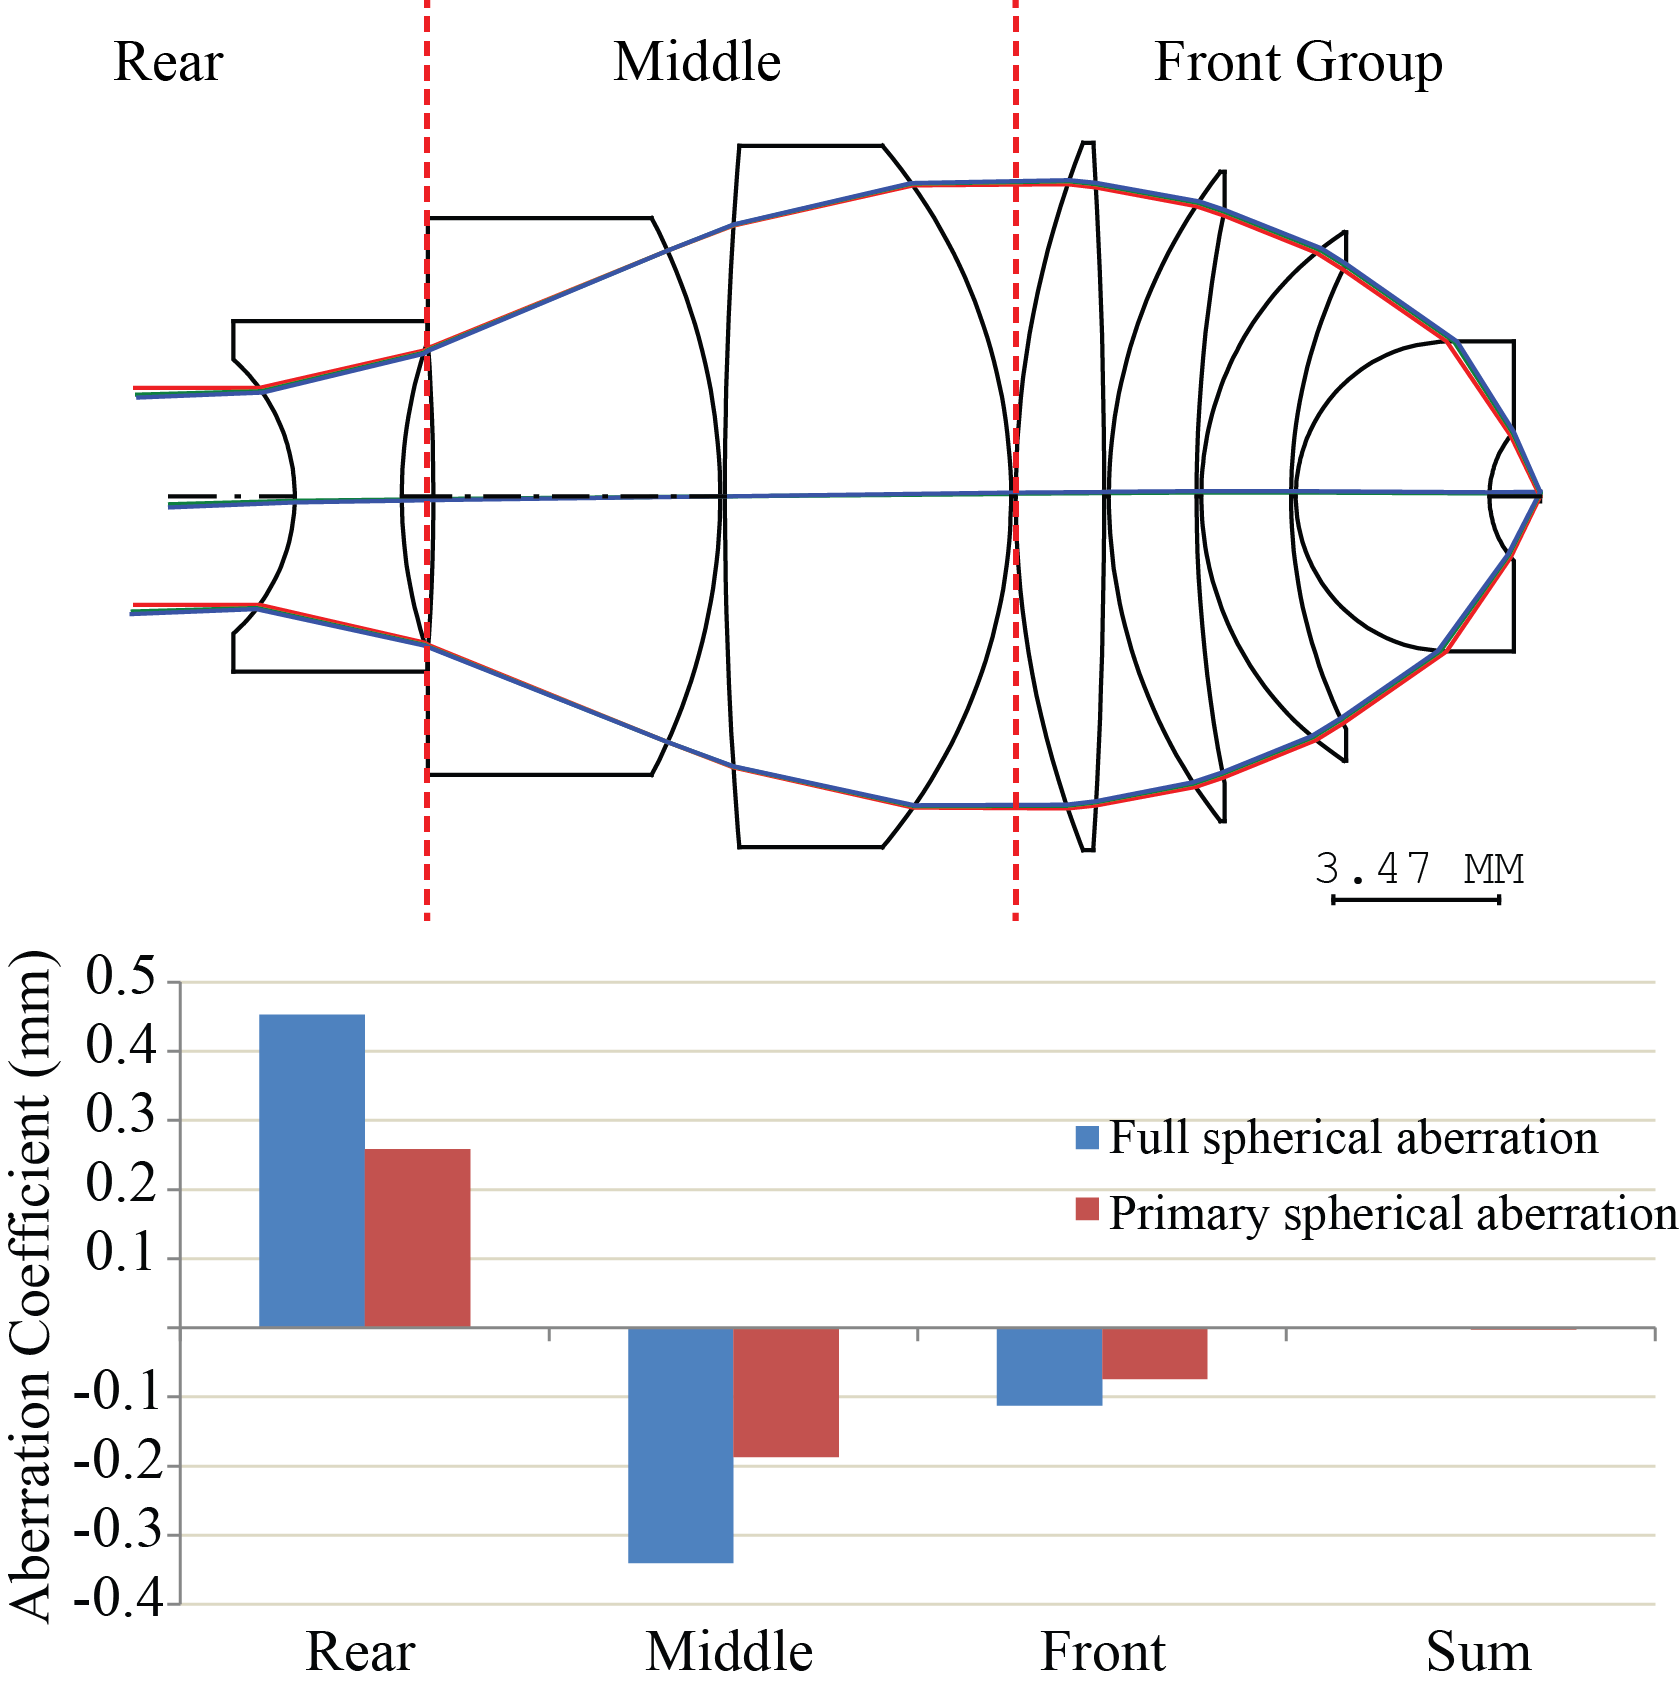
\includegraphics[width=0.55\textwidth]{chapter-4/figures/Vollrath_original.png}
    \caption{System plot of the UV microscope objective \cite{patentvollrath}. The objective can be divided into three function groups, and the rear group and middle group correct the spherical aberration together \cite{ZhangMicroscope2017}.}
    \label{fig: vollrathoriginal}
\end{figure}

The current system already has a good performance and a compact size with the specification listed in Table \ref{table: vollrathspec}. However, if some of the specifications is made more demanding, certain structural modification of the original system is necessary to keep a satisfactory performance. In this section, we investigate how to introduce structural change in the system by using saddle point construction. The main purpose of using saddle point construction is to add lens element in this case. Different from a simple design task, a complex system often needs various constraints in order to fulfill the system requirements. In the following section, we will discuss the use of constraints with saddle point construction in optical design software. 

\subsection{Constraints in optical design software}
The wide angle lens shown in the previous section is a moderate complex system where saddle point construction can be used in limited positions. The system only has one constraint on the effective focal length (EFL) and it was given in as a system solve in CODE v. Given the entrance pupil diameter (EPD), the EFL can be controlled by setting the value of the exit angle of t he marginal ray on the last optical surface. Given the EPD, and the EFL, the exit marginal ray angle $\alpha$ can be set in CODE V as:
\setlength{\belowdisplayshortskip}{5pt}
\setlength{\abovedisplayshortskip}{5pt}
\begin{equation} \label{eq:EFLsolve}
\tan\alpha = \frac{EPD}{2\times EFL}
\end{equation}
\noindent Known system requirements, such as EFL, can be used to force selected parameters to be dependent variables which are solved directly for those system requirements. As other changes are made, these “solves” will keep the chosen requirements satisfied. In Automatic Design, this also makes it possible to reduce the number of independent variables, and thereby save computing time.

However, in lens design practise, most of the system requirements cannot be easily implemented as system solves. Many constraints are then needed for a complex lens design in order to fulfill the various system requirements. In lens design software, the constraints can be set in different ways. Take CODE V as an example, there are four different types of constraints can be used in CODE V as shown in Table \ref{table: codevconstraints}.

%table template
%\setlength{\arrayrulewidth}{.5mm}
%\setlength{\tabcolsep}{18pt}
%\renewcommand{\arraystretch}{1.2}
\begin{table}[h!]
    \centering
    \captionsetup{justification=centering}
    \caption{Different types of constraints in CODE V\cite{codevmanual}}
    \label{table: codevconstraints}
    \vspace{-1em}
    \begin{tabular}{ p{0.31\textwidth} | m{0.45\textwidth} }
    \hline 
    \textbf{Constraint Mode} & \textbf{Explanation}\\
    \hline
    Equality constraint (=) & Always active. Handled with Lagrangian Multiplier Method. Constrains exactly to target value of the constraint.  \\
    \hline
    Inequality constraint (>, <) & Only active when the optimization violates the targeted boundary. Handled with Lagrangian Multiplier Method.\\
    \hline
    Penalty function (PTC) & Only used for targeted constraint.Includes a weighted function in the merit function.\\
    \hline
    Weighted function (WTC) & Only used for targeted constraint. Includes a penalty function in the merit function.\\
    \hline
    \end{tabular}
\end{table}

As we have mentioned in the \colorbox{orange}{previous chapter}, it is necessary to optimize the current optical system to a local minimum for a given merit function in order to operate the saddle point construction. However, it will not be possible for the merit function to locate at the minimum if the constraint is implemented using the method of Lagrange multiplier. One of the advantage of using Lagrange multiplier is that it separates the constraint control from the merit function, allowing the merit function to be based solely upon image quality-related criteria. For the case of an equality constraint, we can write the optimization of the merit function as follows:
\setlength{\belowdisplayshortskip}{5pt}
\setlength{\abovedisplayshortskip}{5pt}
\begin{equation} \label{eq: MFminCon}
\begin{split}
& \text{minimize}\;\; MF(\textbf{x}) \\
& \text{subject to}\;\; g(\textbf{x}) = 0
\end{split}
\end{equation}
\noindent where $\textbf{x} = (x_1, x_2, ..., x_N)$ is a vector describing a point in the $N$-dimensional variable space. $g(\textbf{x})=0$ is an equality constraint that the variables have to satisfy. Given that both $MF$ and $g$ have continuous first partial derivatives, we introduce a new variable $\lambda$ called a Lagrange multiplier and then the Lagrange function can be defined by
\setlength{\belowdisplayshortskip}{5pt}
\setlength{\abovedisplayshortskip}{5pt}
\begin{equation} \label{eq: LagFun}
\mathcal{L}(\textbf{x},\lambda)=MF(\textbf{x})-\lambda\cdot g(\textbf{x})
\end{equation}
Given that $g(\textbf{x})=0$, minimizing $MF(\textbf{x})$ is equivalent to minimizing $\mathcal{L}(\textbf{x},\lambda)$. Therefore, the constrained optimization problem in equation \ref{eq: MFminCon} is converted an unconstrained optimization problem by solving 
\setlength{\belowdisplayshortskip}{5pt}
\setlength{\abovedisplayshortskip}{5pt}
\begin{equation} \label{eq: LagJacob}
\nabla_{\textbf{x},\lambda}\mathcal{L}(\textbf{x},\lambda)=0
\end{equation}
A numerical optimization method can then be applied to minimize $\mathcal{L}(\textbf{x},\lambda)$. From equation \ref{eq: LagJacob}, we can derive
\setlength{\belowdisplayshortskip}{5pt}
\setlength{\abovedisplayshortskip}{5pt}
\begin{subequations} 
\begin{align}
& \nabla_\textbf{x}\mathcal{L}(\textbf{x},\lambda)=\nabla_\textbf{x}MF(\textbf{x})-\lambda\nabla_\textbf{x}g(\textbf{x})=0 \label{eq: LagCondition1} \\
& \nabla_\lambda\mathcal{L}(\textbf{x},\lambda)=g(\textbf{x})=0 \label{eq: LagCondition2}
\end{align}
\end{subequations}
From equation \ref{eq: LagCondition1}, we see that the Lagrange multiplier method converts the original $N$-dimensional problem to $N+1$-dimensional problem by adding one more variable $\lambda$ and one more equation. 
When operating the saddle point construction scan, two extra variables are added to the existing problem. We use $c_{N+1}$ and $c_{N+2}$ as the name of the variables. The scan of the saddle point is to scan the partial derivative of the merit function ($MF$) with respect to the newly inserted variables. This value equals to $\nabla_{c_{N+1}}MF(\textbf{x},c_{N+1},c_{N+2}) \rvert _{c_{N+1}=c_{N+2}}$. The absolute value of the gradient for chosen $c_{N+1}$ or $c_{N+2}$ as an independent variable should be the same. From equation \ref{eq: LagCondition1}, we can derive 
\setlength{\belowdisplayshortskip}{5pt}
\setlength{\abovedisplayshortskip}{5pt}
\begin{equation} \label{eq: nablaMFzero}
\nabla_\textbf{x}MF(\textbf{x}) = 0 \;\; \text{if} \;\; \lambda =0 \;\; \text{or} \;\; \nabla_\textbf{x}g(\textbf{x})=0
\end{equation}
Both of the conditions in equation \ref{eq: nablaMFzero} implies that the space of the constraint overlaps the optimal points in the merit function landscape. However, in practise, it is rarely the case. As a result, we generally threat $\nabla_\textbf{x}MF(\textbf{x}) \neq 0 $ when constraint is implemented using the Lagrange multiplier, and therefore, it will not be accurate to apply saddle point construction scan in this case.
The inequality constraint mentioned in Table \ref{table: codevconstraints} can not be implemented for saddle point construction scan either. The constraint becomes active when the optimization violates the boundary, and remains inactive if the optimization is operated within the defined boundary. Therefore, the merit function landscape is also altered between different status, causing the result of saddle point construction scan to be unreliable. 
Using of penalty function and weighted function in the merit function is possible to combine with saddle point construction scan. Both approaches of implementing the constraints adding extra terms into the merit function with explicit expressions. The merit function is altered, nevertheless, remains unchanged for the following operation. The modified merit function with penalty function term or weighted function term can be written as 
\setlength{\belowdisplayshortskip}{5pt}
\setlength{\abovedisplayshortskip}{5pt}
\begin{equation} \label{eq: MFp}
MF_P(\textbf{x})=MF(\textbf{x})+\sum_{i=1}^{m}P_i(\textbf{x})
\end{equation}
\setlength{\belowdisplayshortskip}{10pt}
\begin{equation} \label{eq: MFw}
MF_W(\textbf{x})=MF(\textbf{x})+\sum_{i=1}^{m}W_i(\textbf{x})
\end{equation}
where the summation indicates that multiple penalty/weighted function can be added. Both approaches for implementing the constraints are essentially identical, and both provide a less rigid control compared to the Lagrange multiplier method. The penalty function mode is ideal for the "soft constraints", which are constraints that have an acceptable range of values \cite{codevmanual}. In CODE V, the expression of the penalty function is not explicitly given. The expression of the weighted function is given as
\setlength{\belowdisplayshortskip}{5pt}
\setlength{\abovedisplayshortskip}{5pt}
\begin{equation} \label{eq: WTC}
W(\textbf{x})=(WTC\cdot \Delta C)^2
\end{equation}
where $WTC$ is the weighting factor set in CODE V, and $\Delta C$ is the departure of the constraints from its target. In the following research on the complex UV microscope objective, the necessary constraints are implemented with the weighted function.

\subsection{Introducing structural change with saddle point construction}
We increased the NA of the microscope objective from 0.90 to 0.95. The rays still can be traced after the modification. The system is then optimized with a wavefront error function. An EFL constraint and a working distance constraint were applied with equality constraint mode. From Table \ref{table: NAchange} we see that the performance of system deteriorates after increasing the NA.

%table template
\setlength{\arrayrulewidth}{.5mm}
\setlength{\tabcolsep}{18pt}
\renewcommand{\arraystretch}{1.2}
\begin{table}[h!]
    \centering
    \captionsetup{justification=centering}
    \caption{Change of the system performance with increasing NA}
    \label{table: NAchange}
    \vspace{-1em}
    \begin{tabular}{ c c c }
    \hline 
     Numerical aperture (NA) & 0.90 & 0.95\\ 
     \midrule
    RMS wavefront error (m$\lambda$) & 48.5 & 111  \\ 
    Strehl ratio at 0 mm & 0.976 & 0.833\\
    Strehl ratio at 0.1 mm & 0.849 & 0.386\\
    \hline
    \end{tabular}
\end{table}




\section{Applying SPC to a lithographic object (extreme complex case)}


%% We need an empty line before the quote environment to work around a bug in
%% the lettrine package, from which the drop command is derived.
\begin{quote}
\texttt{\textbackslash documentclass\{dissertation\}}
\end{quote}
which loads the dissertation template. The template is based on the \LaTeX{} \texttt{book} document class and stored in \texttt{dissertation.cls}. The document class accepts several comma-separated options. By default, hyperlinks are shown in cyan, which is convenient when reading the dissertation on a computer, but can be expensive when printing. They can be turned black with the \texttt{print} option. This will also turn the headers dark gray instead of cyan. Moreover, it will add a 3~mm bleed around the page including crop marks. This will help the printer with the thumb indices, since they run right up to the page borders. Finally, the \texttt{nativefonts} option can be used to override the automatic font selection (see below).

A dissertation is a big document, which makes it easy to miss warnings about the layout in the \LaTeX{} output. In order to locate problem areas, add the \texttt{draft} option to the \texttt{\textbackslash documentclass} line. This will display a vertical bar in the margins next to the paragraphs that require attention.

The contents of the dissertation are included between the \texttt{\textbackslash begin\{document\}} and \texttt{\textbackslash end\{document\}} commands, and split into three parts by
\begin{enumerate}
\item\texttt{\textbackslash frontmatter}, which uses Roman numerals for the page numbers and is used for the title page and the table of contents;
\item\texttt{\textbackslash mainmatter}, which uses Arabic numerals for the page numbers and is the style for the chapters;
\item\texttt{\textbackslash appendix}, which uses letters for the chapter numbers, starting with `A'.
\end{enumerate}
The title page is defined in \texttt{title.tex} in the \texttt{title} folder and included verbatim with \texttt{\textbackslash include\{title/title\}},\footnote{Note that it is not necessary to specify the file extension.} (see below). Additionally, it is possible to include a preface, containing, for example, the acknowledgements. An example can be found in \texttt{preface.tex}. The table of contents is generated automatically with the \texttt{\textbackslash tableofcontents} command. Chapters are included after \texttt{\textbackslash mainmatter} and appendices after \texttt{\textbackslash appendix}. For example, \texttt{\textbackslash include\{chapter-1/chapter-1\}} includes \texttt{chapter-1.tex}, which contains this introduction.

\section{Title Page}

\dropcap{T}{he} title pages are defined in \texttt{title/title.tex}, which you will have to modify according to your needs. Note that these pages are subject to the requirements of the \emph{promotieregelement} and cannot be changed at will. Apart from the names and dates, most of the Dutch text is dictated literally.

Since the thesis title and name of the author appear several times throughout the document (on the title page, but also in, \emph{e.g.}, the preface and cv), special commands are provided so they only have to be specified once. The title (and optional subtitle) can be specified with

\begin{quote}
\texttt{\textbackslash title[Optional subtitle]\{Title\}}
\end{quote}
The name of the author is specified with
\begin{quote}
\texttt{\textbackslash author\{First name\}\{Last name\}}
\end{quote}
Note that the first and last name are separate arguments, since they may be printed in different font shapes. The \texttt{\textbackslash title} and \texttt{\textbackslash author} commands also ensure that the title and author appear in the metadata of the final PDF.

See \texttt{title/title.tex} for detailed documentation on the comment and layout of the title pages. Logos of institutes that have contributed financially to the dissertation may be included on reverse side of the title page. A few example logos can be found in the \texttt{title/logos} folder.

\section{Chapters}

\dropcap{E}{ach} chapter has its own file. For example, the \LaTeX{} source of this chapter can be found in \texttt{chapter-1.tex}. A chapter starts with the command

\begin{quote}
\texttt{\textbackslash chapter\{Chapter title\}}
\end{quote}
This starts a new page, prints the chapter number and title and adds a link in the table of contents. If the title is very long, it may be desirable to use a shorter version in the page headers and the table of contents. This can be achieved by specifying the short title in brackets:

\begin{quote}
\texttt{\textbackslash chapter[Short title]\{Very long title with many words which could not possibly fit on one line\}}
\end{quote}
Unnumbered chapters, such as the preface, can be created with \texttt{\textbackslash chapter*\{Chapter title\}}. Such a chapter will not show up in the table of contents or in the page header. To create a table of contents entry anyway, add
\begin{quote}
    \texttt{\textbackslash addcontentsline\{toc\}\{chapter\}\{Chapter title\}}
\end{quote}
after the \texttt{\textbackslash chapter} command. To print the chapter title in the page header, add
\begin{quote}
    \texttt{\textbackslash setheader\{Chapter title\}}
\end{quote}

If (parts of) the chapter have already been published elsewhere, it is customary to add a reference. This can be done with the special unnumbered footnote command \texttt{\textbackslash blfootnote}. For example,

\begin{quote}
\texttt{\textbackslash blfootnote\{Parts of this chapter have been published in Annalen der Physik \textbackslash textbf\{324\}, 289 (1906) \textbackslash cite \{Einstein1906\}.\}}
\end{quote}
generates the footnote at the beginning of this chapter. Because this footnote is unnumbered, the \texttt{hyperref} package may throw a warning, which safely be ignored.

If multiple people have contributed significantly to this chapter, they can be lister with the \texttt{\textbackslash authors} command. This can be followed by a quotation using \texttt{\textbackslash epigraph} as shown above. Finally, it is customary for a dissertation to include an abstract for every chapter (except perhaps the introduction). This can be accomplished with the \texttt{abstract} environment. The abstract should be followed by \texttt{\textbackslash newpage} to start the chapter text on a new page.

In a dissertation, each chapter has its own list of references. These can be generated with the special command \texttt{\textbackslash references\{dissertation\}} from \texttt{dissertation.bib} at the end of the chapter. Note that this means that you need to run a command like \texttt{bibtex chapter-1/chapter-1} for each chapter. The bibliography style is specified in \texttt{dissertation.bst}, which is a modified version of \texttt{apsrev4-1.bst} (from REVTeX) designed to also display the titles of referenced articles. The template will automatically generate clickable hyperlinks if a URL or DOI (digital object identifier) is present for the reference. Although it is possible to manage the bibliography by hand, we recommend using EndNote (available from Blackboard) or JabRef (available from \url{http://jabref.sourceforge.net/}).

Chapters are subdivided into sections, subsections, subsubsections, and, optionally, paragraphs and subparagraphs. All can have a title, but only sections and subsections are numbered. As with chapters, the numbering can be turned off by using \texttt{\textbackslash section*\{\ldots\}} instead of \texttt{\textbackslash section\{\ldots\}}, and similarly for the subsection.
\section{\textbackslash section\{\ldots\}}
\subsection{\textbackslash subsection\{\ldots\}}
\subsubsection{\textbackslash subsubsection\{\ldots\}}
\paragraph{\textbackslash paragraph\{\ldots\}}
Lorem ipsum dolor sit amet, consectetur adipisicing elit, sed do eiusmod tempor incididunt ut labore et dolore magna aliqua. Ut enim ad minim veniam, quis nostrud exercitation ullamco laboris nisi ut aliquip ex ea commodo consequat. Duis aute irure dolor in reprehenderit in voluptate velit esse cillum dolore eu fugiat nulla pariatur. Excepteur sint occaecat cupidatat non proident, sunt in culpa qui officia deserunt mollit anim id est laborum.

\section{Fonts and Colors}

\dropcap{T}{he} fonts used by this template depend on which version of \LaTeX{} you use. Regular \LaTeX, \emph{i.e.}, if you compile your document with with \texttt{latex}, \texttt{pslatex} or \texttt{pdflatex}, will use Utopia for text, Fourier for math and Latin Modern for sans-serif and monospaced text. However, if you want to adhere to the TU Delft house style, you will need to use \XeLaTeX, as it supports TrueType and OpenType fonts. Compiling with \texttt{xelatex} will use Bookman Old Style for titles, Tahoma for text, Courier New for monospace and Cambria for math. If you want to use \XeLaTeX, but do not want to use the TU Delft house style fonts, you can add the \texttt{nativefonts} option to the document class.

This template supports the use of drop caps, a large colored initial at the beginning of a chapter or section, via the \texttt{\textbackslash dropcap} command:

\begin{quote}
\texttt{\textbackslash dropcap\{L\}\{orem\} ipsum\ldots}
\end{quote}
The first argument is the capital that will be printed on two lines (in the title color), and the second argument is the rest of the word. Depending on the font, the latter may be printed in small caps.

The corporate colors of the TU Delft are cyan, black and white, available, respectively, via \texttt{\textbackslash color\{{\color{tudelft-cyan}tudelft-cyan}\}}, \texttt{\textbackslash color\{{\color{tudelft-black}tudelft-black}\}} (which differs slightly from the default \texttt{black}) and \texttt{\textbackslash color\{tudelft-white\}}. Apart from these three, the house style defines the basic colors
\begin{itemize}
%% Reduce the separation between the items, since this is just a list of words.
\itemsep 0pt
\parskip 0pt
\item\texttt{\color{tudelft-sea-green}tudelft-sea-green},
\item\texttt{\color{tudelft-green}tudelft-green},
\item\texttt{\color{tudelft-dark-blue}tudelft-dark-blue},
\item\texttt{\color{tudelft-purple}tudelft-purple},
\item\texttt{\color{tudelft-turquoise}tudelft-turquoise} and
\item\texttt{\color{tudelft-sky-blue}tudelft-sky-blue},
\end{itemize}
as well as the accent colors
\begin{itemize}
\itemsep 0pt
\parskip 0pt
\item\texttt{\color{tudelft-lavendel}tudelft-lavendel},
\item\texttt{\color{tudelft-orange}tudelft-orange},
\item\texttt{\color{tudelft-warm-purple}tudelft-warm-purple},
\item\texttt{\color{tudelft-fuchsia}tudelft-fuchsia},
\item\texttt{\color{tudelft-bright-green}tudelft-bright-green} and
\item\texttt{\color{tudelft-yellow}tudelft-yellow}.
\end{itemize}

\references{dissertation}

